\chapter{統計モデル}
この章ではついにデータが登場する。データは母集団から無作為抽出によって得られた数値であるとする。
データを大文字の$X_1,X_2,\cdots,X_n$とし、モデルからサンプリングした確率変数を小文字の$x_1,x_2,\cdots,x_n$とする。
統計モデルはデータの出現頻度や統計量などの出現区間などを予測する。
まず、その予測可能なことについて列挙する。モデルとデータが異なる場合つまり、データの出現頻度をデータが予測できない場合に生じることについて説明する。
\begin{SMbox}{統計学に数学は必要か}

    \begin{rightbubbles}{bubblegreen}{Dr$\_$slump7802}{./image/Twitter_logo_PNG/2021_Twitter_logo_blue.png}
        理論や理屈、式の導出をブラックボックス化し、単に『この実験区なら、このデータならこの検定法、このソフト』みたいな講義になっている大学が多いので、統計学嫌いの学生が増えていく。

            \begin{flushright} 
                \small	\url{https://twitter.com/Drslump7802/status/1610784458655006720}
            \end{flushright}    
    \end{rightbubbles}

    \begin{rightbubbles}{bubblegreen}{Dr$\_$slump7802}{./image/Twitter_logo_PNG/2021_Twitter_logo_blue.png}
        よく、『統計学に数学の知識は重要でない』と言い切る人がいるが、それは違うと思う。少なくとも分布のグラフや式がどういう関数であるかは理解する必要がある。

            \begin{flushright} 
                \small	\url{https://twitter.com/Drslump7802/status/1610784907328106496}
            \end{flushright}    
        \end{rightbubbles}

    \begin{rightbubbles}{bubblegreen}{Dr$\_$slump7802}{./image/Twitter_logo_PNG/2021_Twitter_logo_blue.png}
        サンプルデータの条件を把握していることはもちろん前提。
            \begin{flushright} 
                \small	\url{https://twitter.com/Drslump7802/status/1610785188879138816}
            \end{flushright}    
        \end{rightbubbles}

    \begin{rightbubbles}{bubblegreen}{Dr$\_$slump7802}{./image/Twitter_logo_PNG/2021_Twitter_logo_blue.png}
        敵は「検定法のしくみはわからなくてもいいから,実験結果を判定してくれればいいんだ」と平気で学生に語る農学系教員かな。>負の教育拡大再生産
        \begin{flushright} 
                \small	\url{https://twitter.com/Drslump7802/status/1610796746355126275}
            \end{flushright}    
    \end{rightbubbles}

    \begin{rightbubbles}{bubblegreen}{Dr$\_$slump7802}{./image/Twitter_logo_PNG/2021_Twitter_logo_blue.png}
        教員自身はなんとか勉強して使っているけど講義する実力はないし,専門家の非常勤講師を雇う予算もない。だから,数学なしでも成立する学部を目指そうとなっている(苦手だけど勉強するとは大違い)。
        それが現在の地方国立大学農学部の現状。
        \begin{flushright} 
            \small	\url{https://twitter.com/Drslump7802/status/1610799572766580736}
        \end{flushright}    
    \end{rightbubbles}

    \begin{rightbubbles}{bubblegreen}{Dr$\_$slump7802}{./image/Twitter_logo_PNG/2021_Twitter_logo_blue.png}
        農学部や生物学科は,もともと数学から逃避した学生比率が他の理系学部より高いので,数理系基礎科目を教えるのは大変労力を要する。しかし,それが面倒なので,そもそも数学を選択にしたカリキュラムの大学も多く,学生の潜在意識どころが,本当に学部教育が「なんちゃって理系」化している。
        \begin{flushright} 
            \small	\url{https://twitter.com/Drslump7802/status/1610800417763659777}
        \end{flushright}    
    \end{rightbubbles}
\ 
    数学の勉強が少し必要である。
\end{SMbox}

\begin{SMbox}{数学の勉強方法}
    教科書1冊をペンを使って丸写しすることもある。暗記のためではない。手で書いて考えるために行う。
\end{SMbox}
    

\section{正規分布を含んだ統計モデル}
次の3つを仮定したモデルを正規モデルと呼ぶ。
\begin{quote}
    \begin{enumerate}[(1)]
    \item $x_1,x_2,\cdots,x_n, i.i.d. \sim F$
    \item その分布$F$は、正規分布
    \item 正規分布の母数(平均と分散)はそれぞれ$\mu,\sigma^2$。
    \end{enumerate}
\end{quote}
この正規モデルを$M(\mu,\sigma^2)$と書く。$\sigma^2$をある特定の値にしたときのモデルを$M(\mu)$または$M(\mu;\sigma^2)$とし、$\mu$を特定の値にしたモデルを$M(\sigma^2)$または$M(\sigma^2;\mu)$とする。
%モデルに対してある特定の値を当てはめることができるのは、推測したい母集団について、すでに標本を得て、標本分布がわかっている場合である。この母集団を細分化した母集団について、推測した母数を使ったモデルで推測しても良いかを検討するときに、元の母集団に関する知識を使う。

%\subsection{最尤推定量を使ったモデル}
母集団から無作為抽出した標本(データの入った集合)を元にモデルを構築する。正規分布における最尤推定量は、$\mu_{ML}=\bar{X},\sigma^2_{ML}=\frac{1}{n}\sum(X_i-\bar{X})$である。
最尤推定量を元にした統計モデル$M(\mu_{ML},\sigma^2_{ML})$を最尤モデルと呼ぶ。
以下では、正規モデル$M(\mu)$による予測について説明する。

\begin{SMbox}{最尤モデルが最も良い予測をするかはわからない}
赤池は、最尤推定量が母数を推測する上で良い推定量であるとは限らないことを指摘している\cite{1570854174583769344}。
 \begin{quote}
  R.A.Fisherの研究により、観測データxが実際に$p(x|a)$の形の確率分布に従って発生するとき、最尤法が優れた特性を示すことが示された。しかし、応用の場面では、データを生み出す確率的な構造が完全に分かっていることは無いから、Fisherの議論は、最尤法の実上用の根拠を与えない。
 \end{quote}

 本書で扱うデータは、分布形が指定されていないため、最尤推定法で得た母数を取り入れたモデルが予測に適しているとは限らない。
 例えば、中央値などの他の推定量を母数に入れたモデルの方が、良い予測が可能となることがある。

\end{SMbox}



\subsection{データが出現しやすい区間}
ある決められた確率でデータが出現するとモデルが予測する区間を予測区間という。
割合として、よく使われる$95\%$を設定したものを$95\%$予測区間という。
正規分布を含んだモデル$M(\mu)$において、予測区間は比較的簡単に求めることができる。
具体的には、正規分布の規格化を行い、標準正規分布に従うように変換を行い、$\frac{x-\mu}{\sigma}$であるので、予測区間は、
\begin{eqnarray*}
    %-z_{0.05} <\frac{x-\mu}{\sigma} <z_{0.05} \\
    \mu-z_{0.05}\sigma < x < \mu+z_{0.05}\sigma
\end{eqnarray*}
である。この範囲に$95\%$のデータが生じることをモデルが予測する。実際にそのようになるかは不明であり、予測であることを意識した方が良い。

同様に、$68\%$の確率でデータを含むと予測する区間が求められる。
\begin{eqnarray*}
    %-z_{0.05} <\frac{x-\mu}{\sigma} <z_{0.05} \\
    \mu-\sigma < x < \mu+\sigma
\end{eqnarray*}






\subsection{平均値の出やすい区間}
次の統計量$Z$が標準正規分布$N(0,1)$に従うことが、正規分布の再生性によってわかっている。
$$
Z(\bar{x},\mu)=\frac{\sqrt{n}(\bar{x}-\mu)}{\sigma} \sim N(0,1)
$$
ここで$\bar{x}$は、統計モデル$M(\mu)$からサンプリングした標本の標本平均値(データの平均値ではない)、$\mu,\sigma$は統計モデルで設定した母数平均、母数分散。

\if 0
\begin{figure}
    \begin{center}
        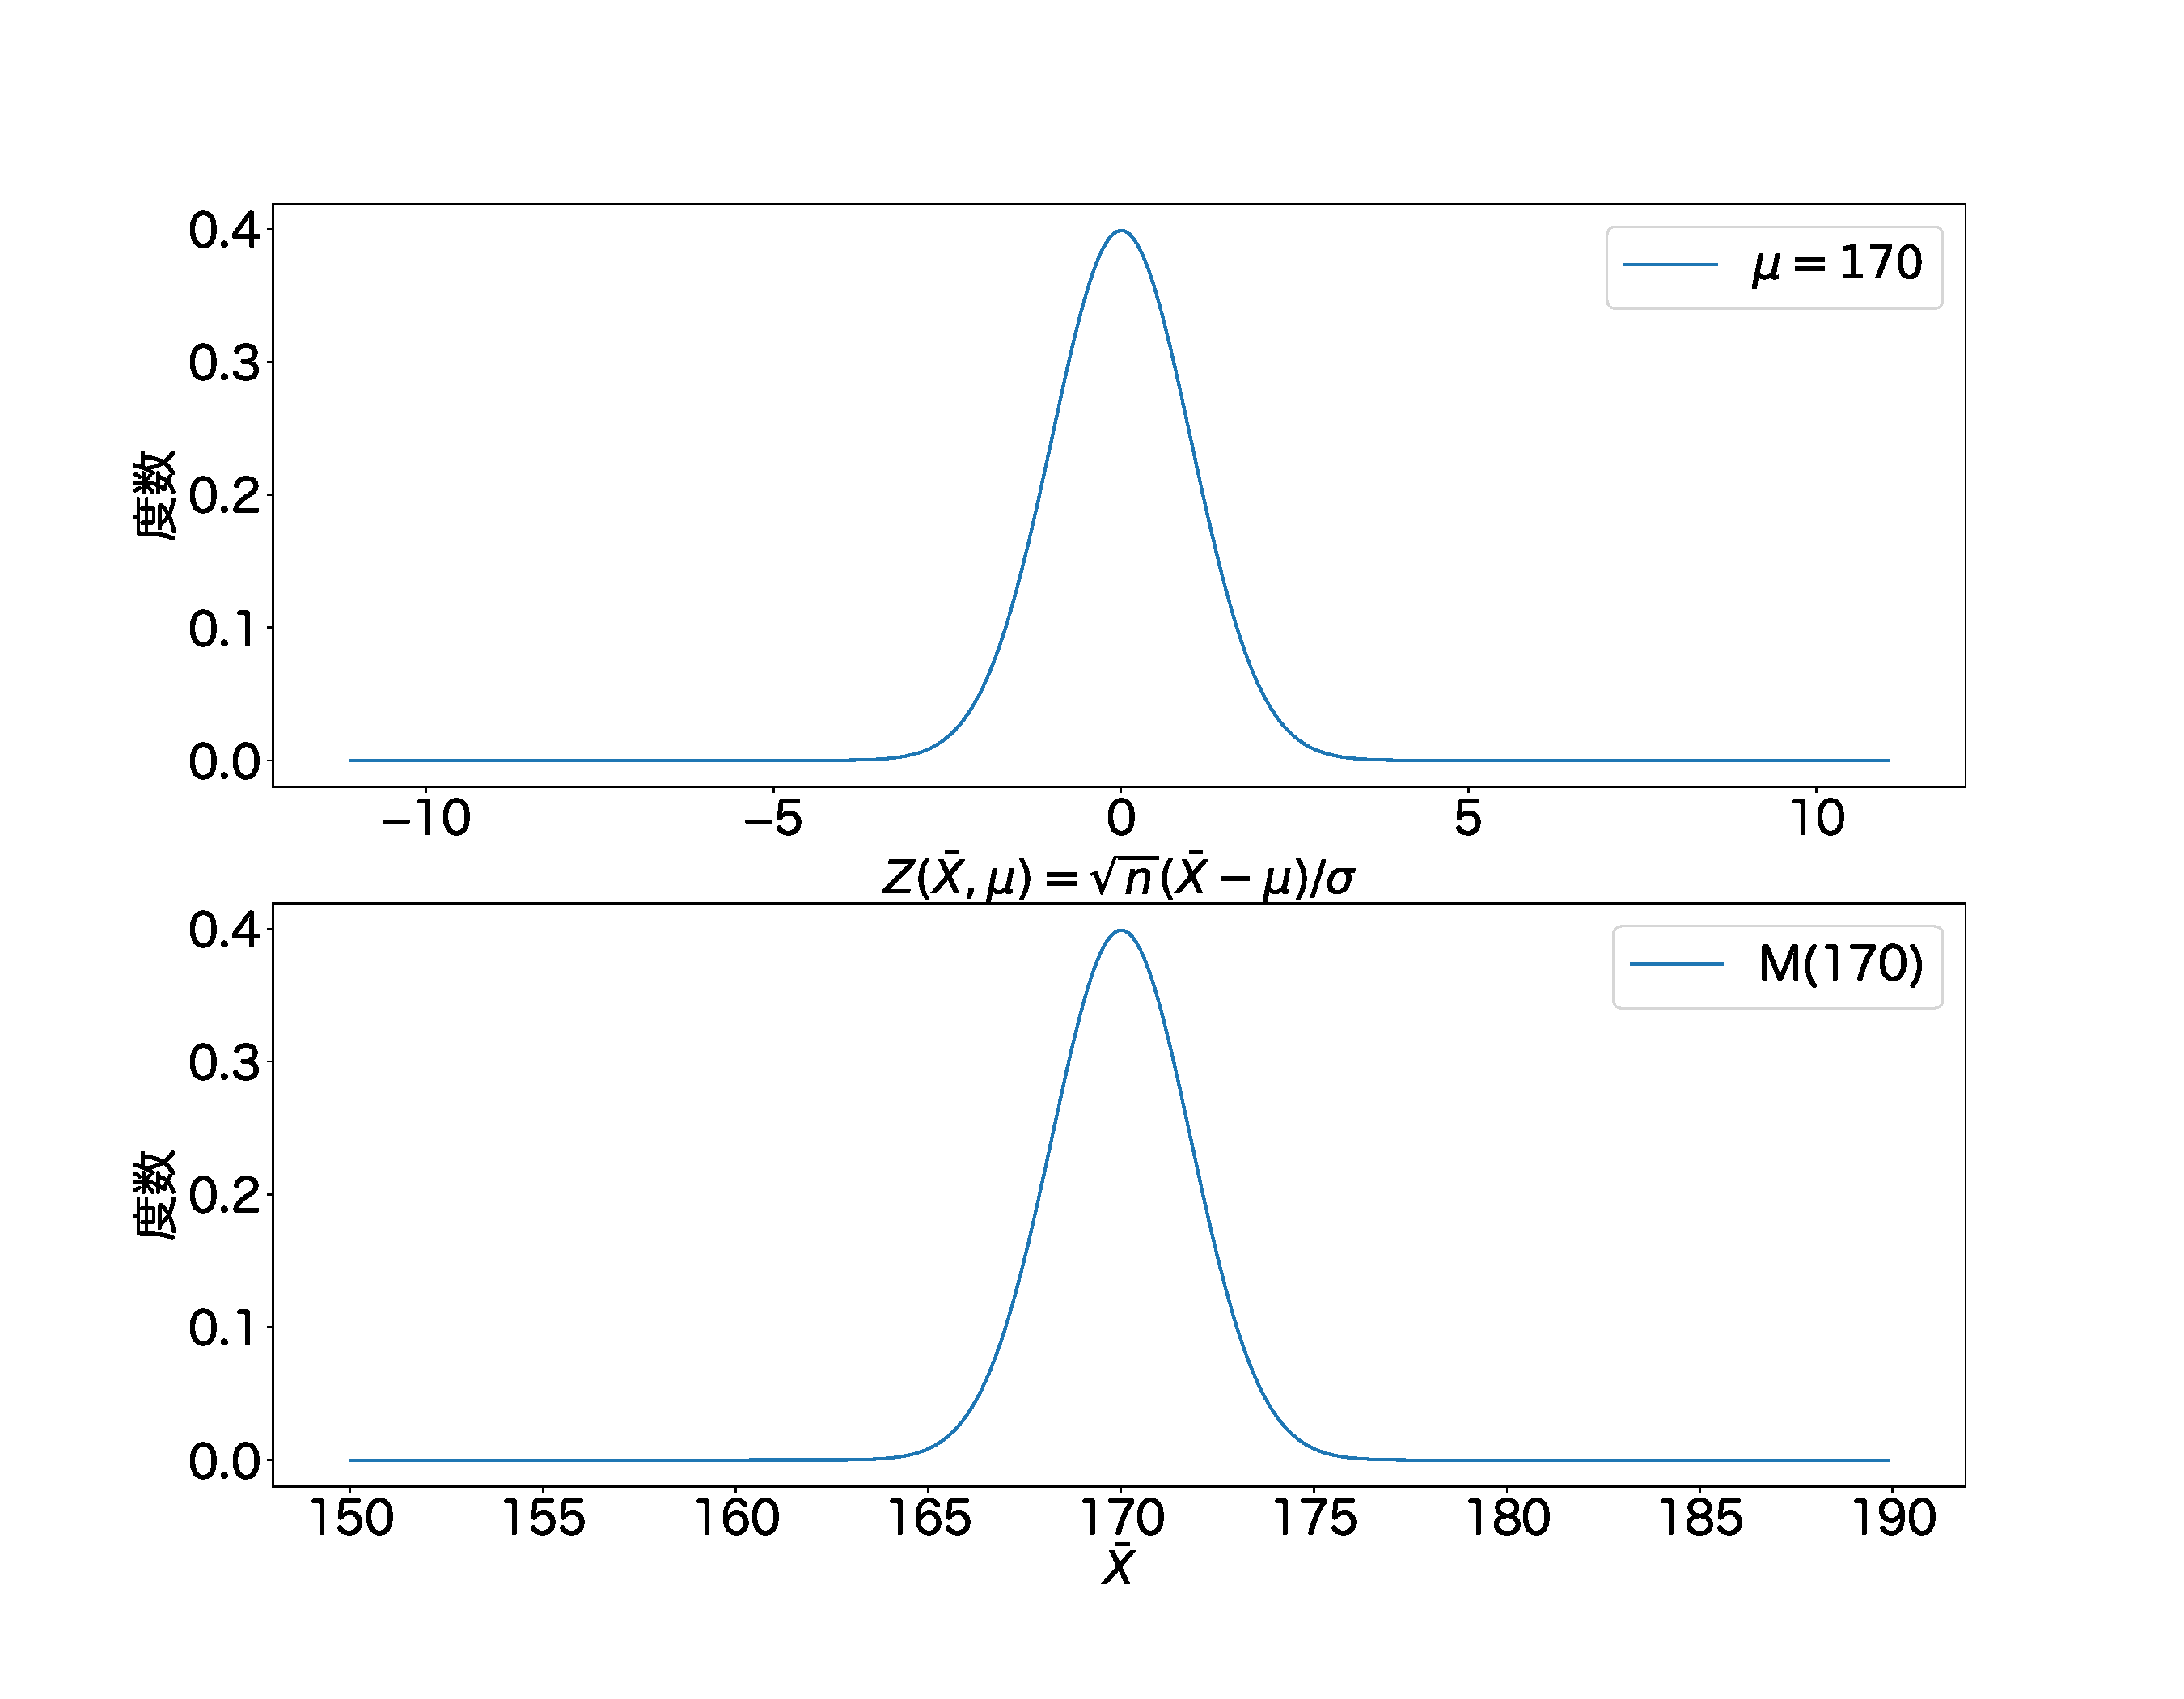
\includegraphics[width=15cm]{./image/03_/normal_Z_frequency.pdf}
        \caption{$M(170;\sigma^2=5.8^2)$における上$Z(\bar{X},\mu)$、下$\bar{x}$。元の統計モデルよりも分散が小さくなることを示さなければならない。TODO}
        \label{fig:cm_standard_normal_distribution}
    \end{center}
\end{figure}
\fi

%$Z$の出現頻度を$Z$または$\bar{x}$の値に応じて書いたものが図\ref{fig:cm_standard_normal_distribution}である。

$Z(\bar{x},\mu)$が、標準正規分布における標準偏差の2倍の範囲($-2 \sim 2$の範囲)にあるあるならば、次の様に式変形できる。
\begin{eqnarray*}
    & -2 < Z(\bar{x},\mu)<2 \\
\rightarrow & -2 < \frac{\sqrt{n}(\bar{x}-\mu)}{\sigma}  <2 \\
\rightarrow & \mu - 2 \frac{\sigma}{\sqrt{n}} < \bar{x} < \mu + 2\frac{\sigma}{\sqrt{n}}
\end{eqnarray*}


\begin{comment}
\begin{equation*}
 \mu - 2 \frac{\sigma}{\sqrt{n}} < \bar{x} < \mu + 2\frac{\sigma}{\sqrt{n}}
\end{equation*}
 
\end{comment}

モデルから決められたサンプルサイズの標本を複数生成し、各標本の平均が$[\mu - 2 \frac{\sigma}{\sqrt{n}} ,\mu + 2\frac{\sigma}{\sqrt{n}}]$の範囲に入るか判定していくと、その頻度は$0.954$である\footnote{数学の記法としては間違えているかもしれないがあえ数式で書くと、$\#\{xはM(\mu;\sigma^2)からサンプリングされた変数の組; Z(x)\in[-2,2]\}/標本数=0.954$である。ここで、$\{\}$は集合であり、$\#{}$は、集合の要素の数。$M(\mu)$からサンプリングした確率変数の組み$x$について、$P(-2\leq z(x)\leq 2)=0.954$でもある。}。これは、標準正規分布の$[-2,2]$の積分値と当然一致する。
この区間を$95.4\%$信頼区間という。

この積分値の小数点$3$桁以降を切り捨てた数値$0.95$になる範囲は、$[-z_{0.025},z_{0.025}]$である。この範囲では、
\begin{eqnarray*}
 & -z_{0.025} < \frac{\sqrt{n}(\bar{x}-\mu)}{\sigma}  <z_{0.025} \\
 \rightarrow & \mu - z_{0.025} \frac{\sigma}{\sqrt{n}} < \bar{x} < \mu + z_{0.025} \frac{\sigma}{\sqrt{n}}
\end{eqnarray*}
である。この区間を$95\%$信頼区間と呼ぶ。

正規モデルにおいて、確率変数が標準偏差の$2$倍を超える値をとる確率は$4.6\%$である。
ある確率変数以上の数値がみつかる確率を$4.6\%$を切上げた$5.0\%$を採用し、
統計量についても、$5\%$となる範囲として$[-z_{0.025},z_{0.025}]$がよく使われる\footnote{正規モデルの場合、標準偏差の$2$倍の区間に確率変数が$95.4\%$ほど見付かるが、あとで説明するように、他のモデルではそのようにならないこともある。}。

%標準偏差の$2$倍の範囲の中で見つかることが大抵であるとことにして、
%統計量についても、$[-2,2]$やなどの範囲が使われる。

\if 0
$Z(\bar{x},\mu)$の$95\%$予測区間が次のように求められる。
$$
-z_{0.025}<Z(\bar{x},\mu)<z_{0.025}
$$
これは、サンプリングされた標本の統計量$Z(\bar{X},\mu)$が$95\%$の確率で得られる範囲である。
科学ではある確率変数がよく出てくる確率として分野を問わず、$95\%$が使われる。
%この値には身長に関する経験を使わずに決定しています。

$Z(\bar{X},\mu)$を式変形することで、標本平均が$95\%$の確率で出現する区間が推定できる。式を変形する。
\begin{eqnarray*}
    & -z_{0.025} < Z(\bar{x},\mu)<z_{0.025} \\
\rightarrow & -z_{0.025} < \frac{\sqrt{n}(\bar{x}-\mu)}{\sigma}  <z_{0.025} \\
\rightarrow & 
\end{eqnarray*}
\fi

\subsubsection{サンプルサイズによる信頼区間への影響}
$95\%$信頼区間の式を見てわかるように、サンプルサイズ$n$が大きくなれば、$\bar{x}$が入る範囲は狭くなる。
信頼区間がサンプルサイズに依存することを数値的に確認する。
図\ref{fig:confidence_interval_n}は、信頼区間が$N$に応じて変化する様子を図示した。

\begin{figure}
\begin{center}
    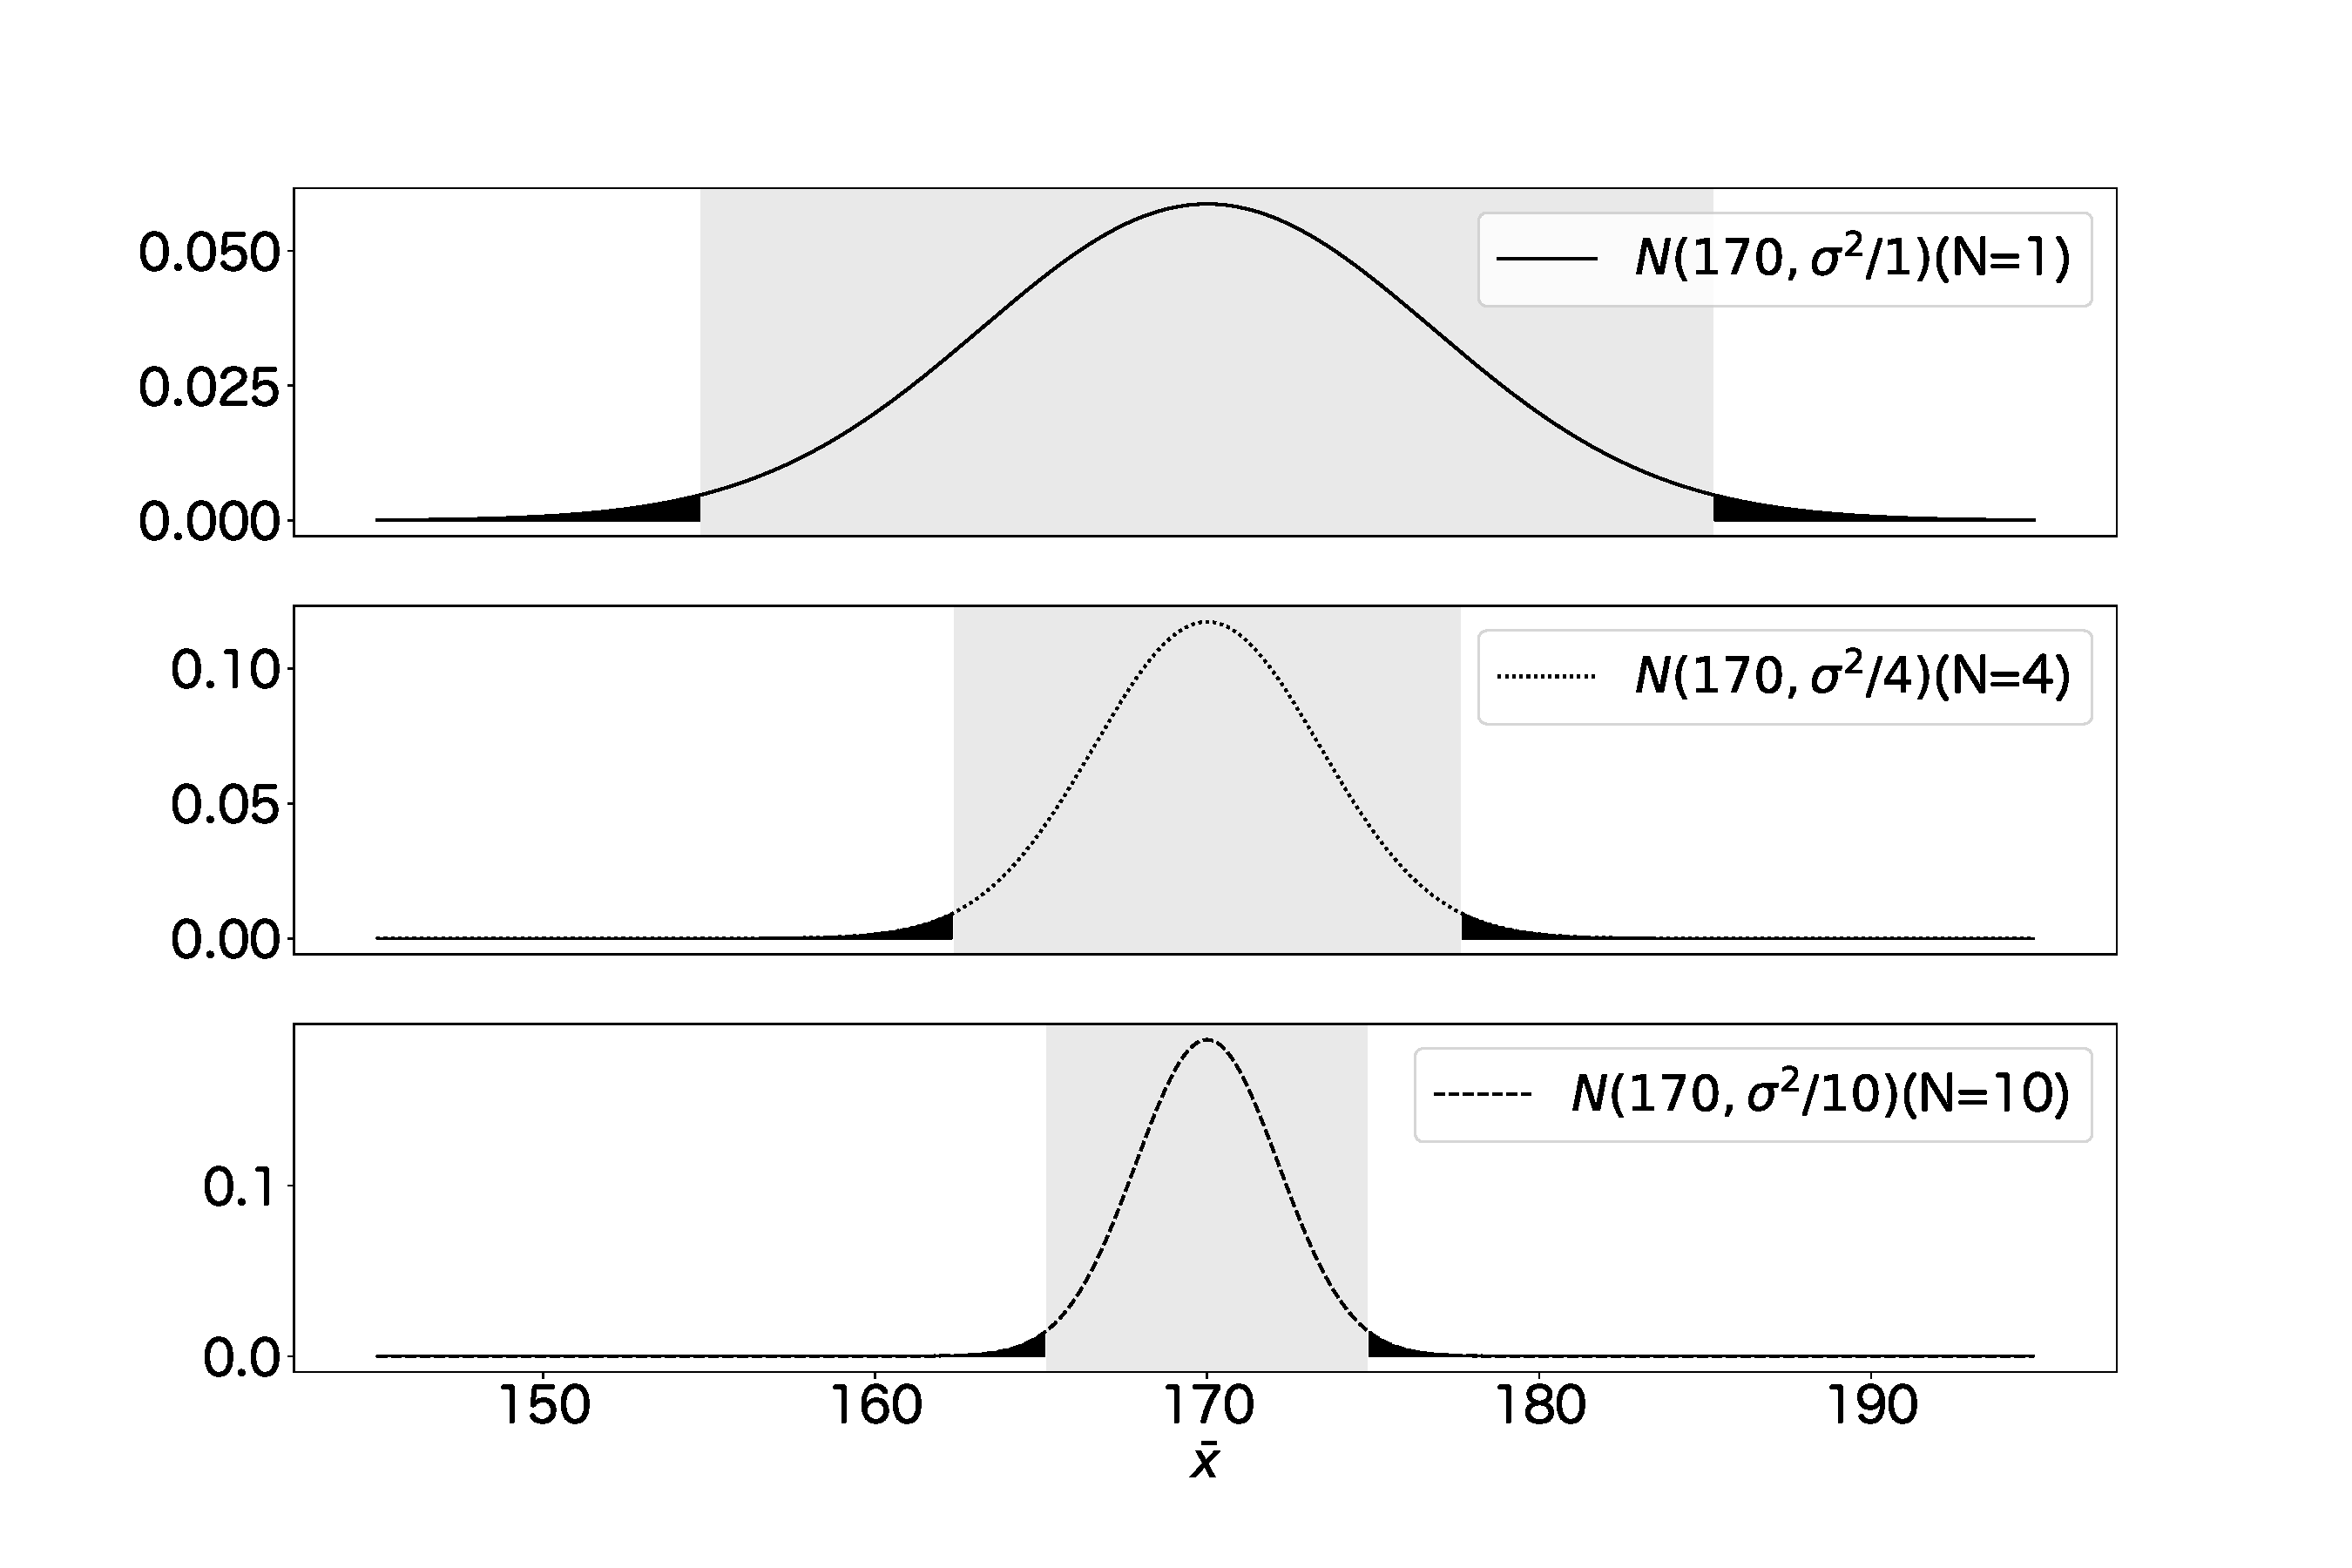
\includegraphics[width=15cm]{./image/03_/confidence_interval.pdf}
%    \caption{信頼区間}
    \caption{モデル$M(170;\sigma^2=5.8)$における(A)$N=1$,(B)$N=4$,(C)$N=10$での$95\%$信頼区間}
    \label{fig:confidence_interval_n}
    \end{center}
\end{figure}


信頼区間の中に標本平均が含まれていることは、標本がモデルにり推測可能であることの証拠の一つになる。
ただし、予測可能かの判断には、複合的に指標を検討する必要がある。

\if 0
\subsection{平均値が出現する区間}
\begin{equation*}
    \mu - z_{0.025} \frac{\sigma}{\sqrt{n}} < \bar{X} < \mu + z_{0.025} \frac{\sigma}{\sqrt{n}}
\end{equation*}
%$Z(\bar{x},\mu)$が$N(0,1)$に従うということから、$Z(\bar{X},\mu)$が$N(0,1)$における出現頻度が計算できる。
この統計モデルからサンプリングした標本の標本平均$\bar{x}$が$95\%$の確率で見つかる範囲のことを$95\%$信頼区間という。これも、モデルの予測である。

一般的な定義として、要約統計量($\bar{x}$など)が$95\%$の確率で見つかることを予測する最小の区間を信頼区間という。

\fi

\if 0
 川久保統計学P.166
 \fi


%![Z値の頻度]()

%$\bar{X}$が$95\%$信頼区間の中に入っていることは、この統計モデル
%信頼区間の中に統計量があれば、
%このことから、統計モデル$M(\mu)$でサンプリングしたときに、$95\%$の確率で、この範囲に平均値$\bar{X}$がえられます。


%標本$1$標本$2$について、これを計算してみる。平均値は、それぞれ172.4, 169.0です。
%\subsection{複数の確率変数から推測する}

\section{二つの正規モデルの比較}
$2$つの正規モデルを、それぞれ次のとおり定義する。
\begin{eqnarray*}
 M_A = M_N(\mu_a,\sigma_a^2) \\
 M_B = M_N(\mu_b,\sigma_b^2)
\end{eqnarray*}
この二つのモデルを比較する。

\subsection{中心間の距離は差の絶対値}
中心間距離は、モデルの中心$\mu_a$から$\mu_b$までの距離として、その差の絶対値で定義する。
\begin{equation*}
 |\mu_a - \mu_b|
\end{equation*}
である。

\subsection{ばらつきの差異は標準偏差の比}
正規モデルにおけるデータのばらつき方の違いは、モデル間の標準偏差の比によって定量的に評価する\footnote{問題:ばらつきを標準偏差の差で定義しないのはなぜでしょう。}。
\begin{equation*}
 \frac{\sigma_a}{\sigma_b}
\end{equation*}
標準偏差の比が$\sim 1$であるならば、だいたい同じような標準偏差であることを示し、$1$より十分大きいならば、モデル$M_b$のばらつきは、モデル$M_A$のばらつきにくらべてかなり大きいことがわかる。

\section{正規モデルにおける中心間の距離(効果量)}
ここでは、分散が等しく、平均が異る二つの正規モデルについて、その間の距離を考える。

\subsection{分散が等しい2つのモデルの効果量}
%ここでは、正規モデル$M_N(\mu;\sigma^2)$について考える。
分散が等しい二つの正規モデル$M_a=M(\mu_a),M_b=M(\mu_b)$とする。
%標準偏差を$1$にすると、それぞれのモデルは、$M_{a'}=M(\frac{\mu_a}{\sigma};1^2),M_{b'}=M(\frac{\mu_b}{\sigma};1^2)$である。
$M_{a'}$の中心から$M_{b'}$の中心への距離は、$D=\frac{|\mu_a-\mu_b|}{\sigma}$となる。
$D$を効果量と呼ぶ。
式を変形すれば、$D\sigma = |\mu_a-\mu_b|$であり、2つのモデルの中心からの距離が標準偏差$\sigma$の$D$個分であることを示す\footnote{効果量の記述をみたら、二つのモデルの確率密度関数があたまに浮かび、それらのピークの間が$D\sigma$くらい離れている図があたまに浮んでくるだろうか}。
%$D=1$であれば、$\sigma$分$M_a$と$M_b$の中心は離れている。
%$D=2$であれば、$\sigma$2つ分$M_a$と$M_b$の中心は離れている。
%$D=0.5$であれば、$\sigma$の半分の距離で$M_a$と$M_b$の中心は離れている。


\subsection{最尤モデルの中心間距離}
二つの母集団A,Bからそれぞれサンプリングを行った標本$X=(X_1,\cdots,X_n),Y=(Y_1,\cdots,Y_m)$について、次の最尤正規モデルを考える。
それぞれの集団にたいして、モデルとして、$M_A(\bar{X},\sigma_{AB}^2),M_B(\bar{Y},\sigma_{AB}^2)$とする。
ただし、ここで$\bar{X},\bar{Y}$はそれぞれ標本$X,Y$の平均値であり、$\sigma_{AB}$は、二つの標本からプール(重み付き平均)した標準偏差である。
具体的には、
\begin{eqnarray*}
 \sigma_{AB}^2 &=& \frac{n\sigma_A^2+m\sigma_B^2 }{n+m}\\
 & = & \frac{n\times \frac{1}{n}(\sum_i^n (X_i -\bar{X})^2)  }{n+m} + \frac{m\times \frac{1}{m} (\sum_i^m (Y_i -\bar{Y})^2)  }{n+m} \\
 & = & \frac{(\sum_i^n (X_i -\bar{X})^2)  }{n+m} + \frac{(\sum_i^m (Y_i -\bar{Y})^2)  }{n+m}
\end{eqnarray*}
である。最尤モデル$M_A,M_B$の中心からの距離を、標準偏差で割った量を$D$とする。$D$を具体的には、
\begin{equation*}
 D = \frac{|\bar{X}-\bar{Y}|}{\sigma_{AB}}
\end{equation*}
である\footnote{ここで考えた$D$は一般には、Cohen's Dと呼ばれている量と一致する。ただし、モデルを考えずに定義するのがならわしである。}。いつでも効果量を報告することは推奨できない。このことを調べてみる。

\subsection{分散が等しいとするとおかしな例}
分散の異る標本を得た場合、効果量の意味がとりにくいことを示す。

ふたつの条件$A,B$で何らかの実験を行ったとして\footnote{実際には、正規分布$N(0,20^2),N(10,10^2)$からサンプルサイズ$100$の標本を得た。}、それぞれで表\ref{table:cohen_d_pooled_std_model}のような統計量が得られた。
それぞれの条件で、正規モデルで推測してみても良さそうだと判断したとする\footnote{ここで複数の疑問が生じる。平均はプールしないのは理由をおおよそ理解できるが、分散をプールしたほうがいい理由は自明ではない。データが二つの標本分散が同じ程度であることを示し、それらを統一したモデルで詳細をしらべたいという意思の部分がある。}。

\begin{table}[hbtp]
 \caption{条件$A,B$で得られた標本の統計量}
 \label{table:cohen_d_pooled_std_model}
 \centering
\begin{tabular}{lrr}
\hline
{} &   条件$A$ &   条件$B$ \\
%\midrule
\hline
サンプルサイズ & 1000 & 1000 \\
平均  &    0.78 &   10.27 \\
分散   &   19.63 &   10.31 \\
最小値   &  -61.08 &  -21.53 \\
25\%   &  -12.00 &    3.53 \\
50\%   &    0.83 &   10.31 \\
75\%   &   14.08 &   17.30 \\
最大値   &   79.17 &   44.33 \\
%\bottomrule
\hline
\end{tabular}
\end{table}


分散の違いを示すため、分散比を計算すると、分散の比は、$\frac{19.63}{10.31}\sim 2$である。分散が同じとしてモデルを作れば、それぞれの標本を予測しにくくなると考えられる\footnote{分散がいっぽうの$2$倍程度違うので、同じ分散としてモデルを構築し、データを予測できるとは考えにくい。}。この判断を行えば、効果量によりモデル間の距離を測るのも難しいと判断ができる。
あえてここでは、同じでもええかと実験者が考えた場合、モデルとデータが乖離してしまうことを示す。

プールした分散は、$\sigma_{AB}=16.37$である。プールした分散を用いたモデルは、それぞれ
\begin{eqnarray*}
 M_A(0.78,16.3^2)\\
 M_B(10.27,16.3^2)
\end{eqnarray*}
である。
最尤モデルはそれぞれ
\begin{eqnarray}
 M_A^{\rm{ML}}(0.78, 19.63^2)\\
 M_B^{\rm{ML}}(10.27, 10.31^2)
\end{eqnarray}
である。
それぞれのモデルがデータをよく予測するかを確認する。
表\ref{table:cohen_d_model_data_diff}は、それぞれのモデルにより推定した、$1$標準偏差,$2$標準偏差の区間に期待される量のデータが含まれているかを調べた結果である。
それぞれの実験において、最尤モデルは、モデルが期待する区間に対応する量のデータが含まれている。それぞれ、$694$個と$671$個であり、モデルの予測と十分近いといってもいいだろう。
一方で、プールされた分散を用いたモデルは明かに、予測と乖離する。これは、二つの条件の間で分散が異ることで、モデルの予測精度が低下しているからである。
以上のことは、データとモデルが乖離しており、プールしたモデルを使わない方が良いという証拠の一つになる\footnote{実践(論文)では、ここまで考察しているのかが府明瞭なことが多い。}。

\begin{table}[hbtp]
 \caption{モデルとデータの乖離に関する調査}
 \label{table:cohen_d_model_data_diff}
 \centering
\begin{tabular}{lrr}
\hline
{}条件$A$ &   $68\%$ &   $95.4\%$ \\
\hline
 $M_A^{\rm{ML}}$& $694$  & $950$ \\
 $M_A$ & $604$  & $902$ \\
\hline \\ \\
\hline
{}条件$B$ &   $68\%$ &   $95.4\%$ \\
\hline
 $M_B^{\rm{ML}}$& $671$  & $958$ \\
 $M_B$ & $892$  & $999$ \\
\hline
\end{tabular}
\end{table}


図\ref{fig:cohen_d_pooled_std_model}には、それぞれのモデルにおける確率密度関数を示した。現状の解析では、$(c)$の最尤モデルがもっともデータを説明できている。
このモデルをなかったことにして、$(d)$を採用し、(d)中の矢印間の距離を標準偏差で規格化した量を効果量とよぶことにする。
効果量がデータを予測できないモデルの中心間距離を標準偏差で規格化した量になる。予測に適さないモデルに関する性質となっており、これでは効果量の意味を捉えにくい\footnote{多くの論文では、データが正規分布に近いのか、分散が等しいのか評価していないので、効果量が何を示しているのか判断つきにくい。ただし、コントロール郡と対照郡とで分散がほとんど同等であったという実験も多いため、分散の評価をしないのかもしれない。}\footnote{さまざまなモデルで調べてみたという言い訳も考えられるが、明かにデータを説明できないモデルの性質を示すことに意味があるのだろうか}\footnote{効果量を大きくするにはどうしたらいいだろうか?観測データの中心から外れた大きめの値を抜けば、分散が小くなり、効果量は大きくなる。やりたいほうだいだ!}\footnote{問題:もっとデータに対して適切な分散は存在するだろうか?例えば、$\bar{z}=n\bar{x}+m\bar{y}$として、分散を$\sigma^2 = \frac{\sum^n(x_i-\bar{z})^2 + \sum^m (y_i-\bar{z})^2}{n+m}$とし、それぞれのモデルを構築してみてはどうだろう。データにフィットしているだろうか?不偏分散を採用して、モデルを構築したものだとどうだろう。データを説明できるだろうか?}。

\begin{figure}
 \begin{center}
  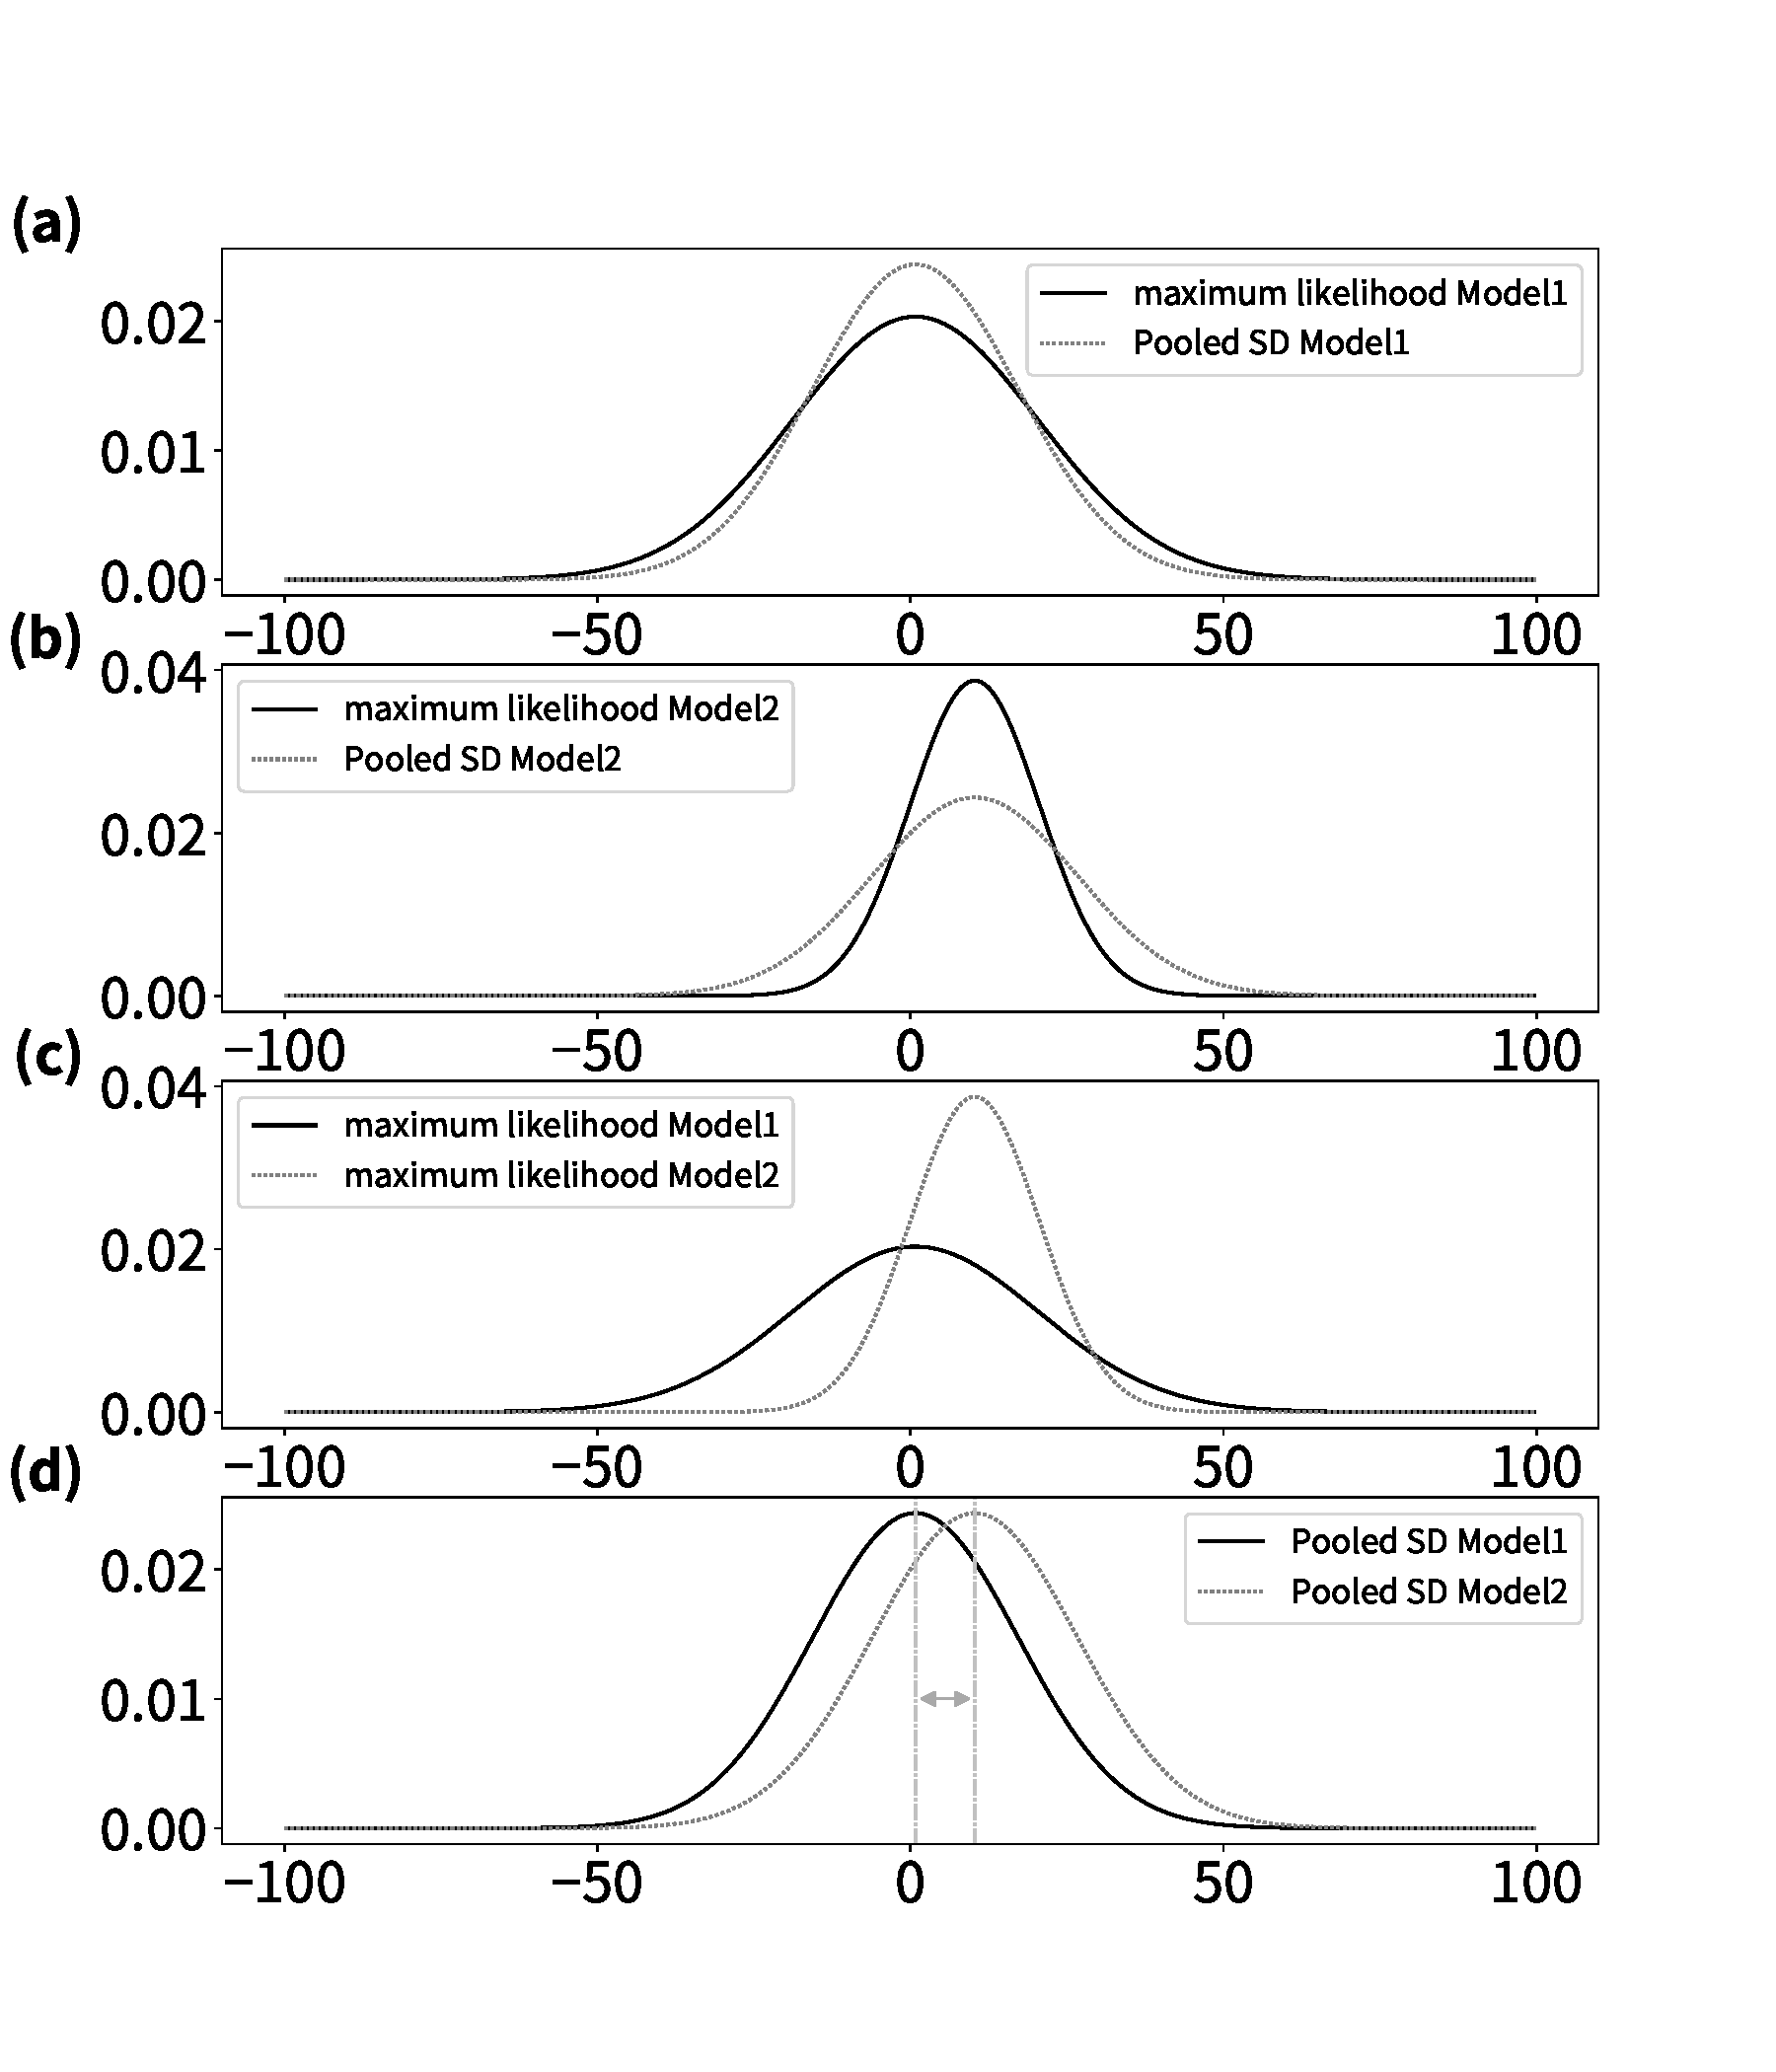
\includegraphics[width=12cm]{./image/12_/cohen_d_pooled_std_model.pdf}
  \label{fig:cohen_d_pooled_std_model}
  \caption{(a,b)条件$A,B$に対する最尤モデルとプールされた分散によるモデルの確率密度関数。(c)条件$A,B$の最尤モデルの確率密度関数。(d)プールされた分散のモデル。矢印間の距離を標準偏差で割った値が効果量。実際に知りたいのは、(c)における二つのモデルの性質の差異。}
 \end{center}
\end{figure}

\subsubsection{正規モデル以外の場合}
正規モデルではデータとの乖離が激しく、正規分布以外の分布形を仮定したモデルを使った場合を考える。例えば、指数分布を仮定した場合、分散をプールしてしまえば、平均も一致するので、効果量を定義通りに計算すると常に$0$である。正規モデルがデータと乖離していない場合には使える量である\footnote{ただの分散の等しい二つの統計モデルの中心間の距離が標準偏差何個分かを示しているにすぎない。}。


\if 0
$D$は、$\sigma$で規格化したことにより、標準正規分布の標準偏差の尺度を使って、モデル間差異を示すことができる。
例えば、$D=1.0$であれば、$\mu_a\pm 1$の当たりに$M_b$の中心があることを示す。
これは、$M_b$における平均値$\mu_b$以上の値が$M_a$において出現するのは、標準正規分布におけるパーセント点1の上側確率を計算すれば、およそ、$\varPhi(1)\sim0.168$である。
$D=0.5$であれば、同様の計算をすれば、$\varPhi(0.5)=0.308$である。
$D=0.01$であれば、$\varPhi(0.01)=0.496$である。
%このモデルの中心間の距離は、$|\mu_a-\mu_b|$である。
\fi


\begin{SMbox}{Normal(正規)分布}
 Normal(正規)分布はもともとガウス分布という名前がついていた。
 同時期に複数人がNormalとよんだ。1873年に哲学者のチャールズ$\cdot$サンダー$\cdot$パース、$1877$年にドイツの統計学者ヴィルヘルム$\cdot$レキシス、
 そして、先に紹介したゴールトン。

\begin{comment}
 さまざまざ集団の変異が、正規分布的であったという結果から、これから調べる集団でも同様の性質があらわれるという保証はどこにもない。
 実際、体重の分布や年収の分布は正規分布的ではない。
正規分布が正常であるという保証はどこにもなく、データとモデルの比較により、変異の特徴をしらべることが求められる。

ではなぜ、データ正規モデルを使うのかというと、変異の特徴がわからないので、取り敢えず正規モデルを構築する。
 データと正規モデルを比較し、うまくデータを推定できないなら、他のモデルを構築する。

 実践的には、変異の特徴に興味をもつ科学者は少く、平均値の変異を議論することが多い。
%正規モデルではないモデルを使うことで良い推定が可能である。
  %計測技術の進歩により、計測の誤差は小くなり、緻密な計測が可能になっている。これまで見えなかった変異の詳細も得ることができるようになる。
\end{comment} 
\end{SMbox}


\section{指数分布を含んだ統計モデル}
\begin{quote}
    \begin{enumerate}[(1)]
    \item 独立同分布
    \item その分布は、指数分布$(\lambda\exp{(-\lambda x)})$
    \item 指数分布の母数は$\lambda$
    \end{enumerate}
\end{quote}
このモデルを$M_E(\lambda)$とする。
このモデルの$95\%$予測区間は、
\begin{equation*}
    [\frac{1}{\lambda} \log\frac{1}{1-\alpha/2} ,\frac{1}{\lambda}\log\frac{\alpha}{2} ]
\end{equation*}
である。
%指数モデルにおける$95\%$予測区間は、構成が難しいようなので、省略する\footnote{どうすれば求められるのか、わからない}。
$95\%$信頼区間は式\ref{exp_model_confidence_interval}である。


\subsection{信頼区間の近似}
$95\%$信頼区間(式\ref{exp_model_confidence_interval})を近似的に求める方法がある。
中心極限定理を使う。このモデルでは、サンプルの平均および分散は、$E[x]=\frac{1}{\lambda},Var[x]=\frac{1}{\lambda^2}$である。このとき、中心極限定理により、$\bar{x}\sim N(E[x],Var[x]/n)$である。よって、$95\%$信頼区間は、
\begin{equation*}
\frac{1}{\lambda}-z_{0.05}\frac{1}{\sqrt{n}\lambda}<\bar{x}<\frac{1}{\lambda}+z_{0.05}\frac{1}{\sqrt{n}\lambda}
\end{equation*}
である。

解析的に求めた信頼区間と中心極限定理による近似的な信頼区間を比較する(図\ref{fig:model_predict_CI_interval})。
$\lambda=10$としたので、平均は全て$10$である。
$N$が小さいと、解析と近似での信頼区間に差が生じている。近似的な信頼区間は、$0$よりも小さな値も出現することを予測している。平均$10$の指数モデルでは、平均が$0$以下になることはない。このように、モデルの想定しない区間も信頼区間に含めている。
$N$が大きくなると、解析と近似での信頼区間が一致しやすくなる。
%これは、中心極限定理の帰結から当然である。

\begin{figure}
 \begin{center}
  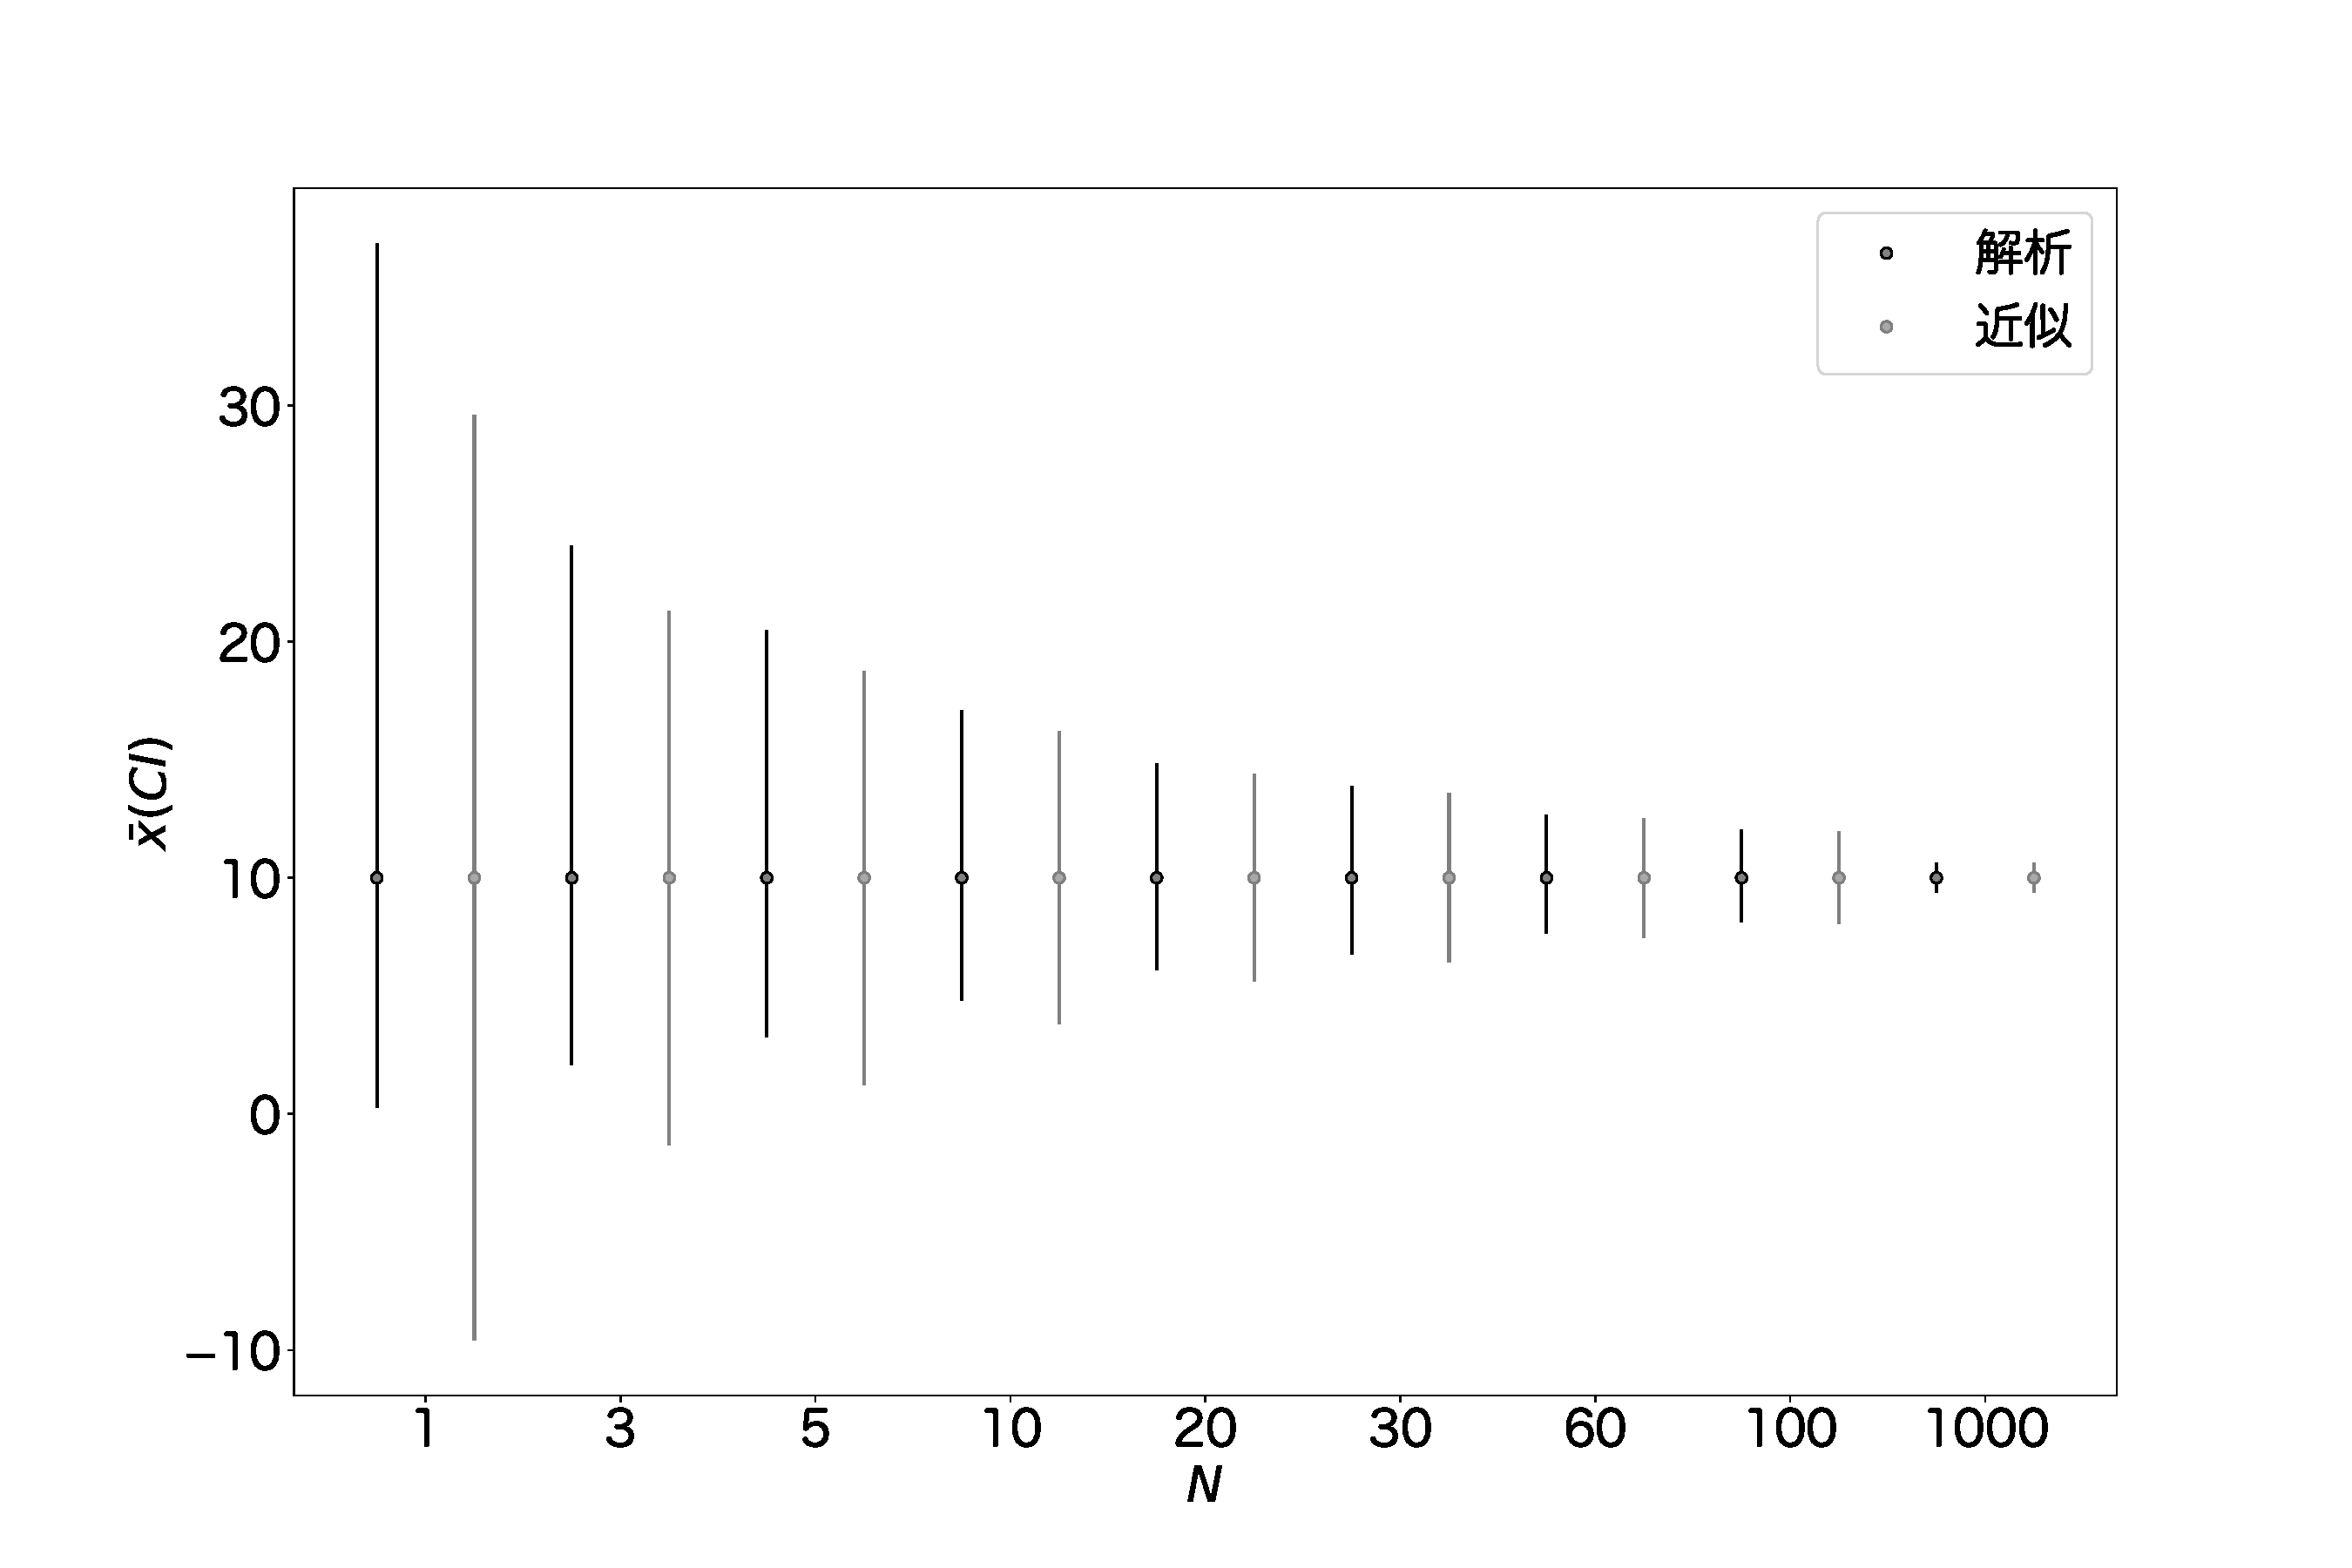
\includegraphics[width=15cm]{./image/12_/confidence_expon_interval.pdf}
  \label{fig:model_predict_CI_interval}
  \caption{解析的な信頼区間と近似によって求められた信頼区間。$1/\lambda=10$とする。横軸にサンプルサイズ。縦軸に、平均値。エラーバーは信頼区間(CI)。}
 \end{center}
\end{figure}

\if 0
\section{モデルの選択}
データの分布とモデルの分布が一致しているとき、そのモデルの予測も当たりやすい。
例えば、データがある値の周りに対称に分布していないにもかかわらず、正規モデルを使うと、その予想は当たりにくい。
モデルの予測が当たると思わせるには、標本分布に関する知識が必要であり、その知識があれば、モデルの予測が当たりやすいと他の人に説得しやすくなる。
このことから、まず、標本分布に関する、適当な分布の形(母数を含めた)を探索する必要がある。
モデルを選択できるほどのサンプルサイズを集めて、母集団を予測しやすいモデルを決めることで、予測が当たりやすくなると思える\footnote{実際に予測が当たるかはわからない}。
%なり、モデルの予測を信頼しやすくなる。

実際の研究では、実験のコスト増加のことを考慮すると、事前実験により標本分布を調べることは、ほとんど不可能である。
そこで、何も事前研究がないなら、何のモデルと比べてみたいのかを決めておき、その予想モデルとデータを比較するのも良い。
\fi

%モデルがデータを捉えていない場合でも、中心極限定理により信頼区間はそれなりに当たることが多い。
%ただし、予測区間が現実をよく捉えているかはわからない。

%正規モデルにより推測を行うことを検討するのも良い。
%実験前の事前計画によって決めたモデルを、実験データを見た後に変更することは行ってはいけないことになっている。

%ここで、現状のデータからモデルを選択したとして、その予測が当たるかはわからない。
%サンプルサイズが小さいとき、予測が当たりそうなモデルを選ぶことが難しい。
%事前実験やこれまでの研究結果から推測し、モデルの分布と標本分布が一致していそうなモデルを選ぶことになる。


\section{対数正規分布を含んだ統計モデル}
次の3つを仮定したモデルを対数正規モデルと呼ぶ。
\begin{quote}
    \begin{enumerate}[(1)]
    \item $x_1,x_2,\cdots,x_n, i.i.d. \sim F$
    \item その分布$F$は、対数正規分布
    \item 対数正規分布の母数(平均と標準偏差)はそれぞれ$\mu,\sigma$。
    \end{enumerate}
\end{quote}

この対数正規モデルを$M_{\log}(\mu,\sigma)$と書く。
最尤正規モデルの母数は、
\begin{eqnarray*}
 \mu_{ML} = \frac{1}{n}\sum_{i=0}^{n} \log x_i \\
 \sigma^2_{ML}= \frac{1}{n}\sum_{i=0}^{n} (\log x_i  -\mu_{ML})^2 \\
\end{eqnarray*}
であり、そのモデルを$M^{ML}_{\log}(\mu_{ML},\sigma_{ML})$と書く。



\section{モデルとデータの乖離を調べる}

\subsection{チェビシャフの不等式}
\begin{lemm}
 確率変数$x$が平均$\mu$,分散$\sigma^2$であるとき、次の不等式が成り立つ。
 \begin{equation*}
  P(|X-\mu| \geq k\sigma) \leq \frac{1}{k^2}
 \end{equation*}
ここで、$k$は任意の正の数。不等式の不等号を変えてやると、
 \begin{equation*}
  P(|X-\mu| \leq k\sigma) \geq 1-\frac{1}{k^2}
 \end{equation*}
\end{lemm}
この不等式を使えば、標準偏差をばらつきの基本単位として、その単位の中にどれくらいデータが入るのか推定できる。例えば、$k=2$の場合を記述すると、
 \begin{equation*}
  P(|X-\mu| \leq 2\sigma) \geq \frac{3}{4}
 \end{equation*}
$\mu$から$2\sigma$の範囲の中にある確率変数は、$75\%$程度より多いことを示している。
\begin{lstlisting}
 x = np.arange(0,12,0.01)
 y = np.sin(x/(2*np.pi)*20)
 plt.plot(x,y)
 plt.show()

 np.random.shuffle(y) # やらなくてもよい

 df = pd.DataFrame(y,columns=['x'])
 sns.swarmplot(data=df, y="x");plt.show()

 mu,sigma = np.mean(df['x']),np.std(df['x'])
 x = df['x']
 print(mu,sigma)
 print(np.sum( np.abs(x-mu)<=2*sigma )/len(x), np.sum( np.abs(x-mu)>=2*sigma )/len(x))
\end{lstlisting}
最後行の出力は、$3/4$以上、$1/4$以下であり、計算してみると、期待通り$1,0$が出力されている。




%\section{モデルでデータを推測可能}
\subsection{正規モデルの場合}
正規モデル$M(\mu)$によりある現象を予測できるのかを考える。
ここで、サンプルサイズ$1$の標本を使によって、モデルの良さを考察できるかを考える。
$M(\mu)$であれば、$95\%$の確率で、$\mu-\sigma z_{0.025}\sim \mu+\sigma z_{0.025}$の間でデータが見つかることを予測する。
この中に入っていることが予測可能の目安の一つにはなる。
サンプルサイズが小さい場合では、標本分布の形がどの分布に適合するのかを推測しにくので、このモデルが現実を予測していると言い切ることはできない。

標本全体を使えるのならば、
\begin{enumerate}
 \item 母数平均よりも小さいまたは大きな点が半分程度であることを予測している(平均に対してデータが対称的に分布している)。
 \item 標準偏差の内側、言い換えれば、$[\mu-\sigma<x<\mu+\sigma]$の中にあるデータの数は$68\%$程度。
 \item $[\mu-2\sigma < x < \mu+2\sigma]$の中にあるデータの数は$95.4\%$程度。
\end{enumerate}
などがデータに当てはまるのかを調べる。


%我々の科学では、モデルが現象を推測可能であるかをたったひとつの値から判定しない。

%$\sigma^2=1$とすると、$95\%$の確率で、確率変数は、$\mu-1.96\sim\mu+1.96$の間で見つかる。
%$\mu=0$なら、$x=0.1$は、この区間の中にあるので、$x$は、$N(0,1)$では良く見つかる値になる。
%この基準では、複数の$\mu$で$x=0.1$はよく見つかる範囲に入る。例えば、$\mu=0.1$でも良く確率変数が見つかる区間は、$-1.85\sim 2.05$なので、確率変数は、$N(0.1,1)$に従うとしても問題ない。
%$x=0.1$がその区間に入らない母数は、$\mu=z_{0.025}+0.1$のときで、区間は$0.10003\sim4.01$で、この区間に$x$は入ってません。
%これを言い換えれば、母数$x-z_{0.025}\leq\mu\leq x+z_{0.025}$の間でよくある値になり、この間から外れた母数をもつ$N(\mu,1)$に従っていいないと推測できる。

\if 0
例えば、$x=1.97$が得られたとすると、$N(0,1)$のよく出る値の範囲は、$-1.96\sim1.96$であることから、母数$0$ではないと判断できます。
一方で、$N(0,1)$で$x=1.97$は、サンプルサイズが$20$であれば、そのうち$1$回は、$1.97$をとる値です。もしももう一度サンプリングできたとして、その値が$0$になることもあり得ます。
以上のことから、$1$回のサンプリングだけで判断しません。
\fi

\subsection{母集団の標本が指数分布的に分布していた場合}
母集団の分布形と統計モデルに含まれている確率分布関数が著しく異なる場合を考える。
母集団分布として、指数分布を仮定する。これは、自然から指数分布的なデータが得られたときのことを想定している。
これを予測するモデルを正規モデルとしてみる。

最尤モデルは、$M(\mu_{ML},\sigma^2_{ML})$である。ここから、
\begin{eqnarray*}
    %-z_{0.05} <\frac{x-\mu}{\sigma} <z_{0.05} \\
    \mu_{ML}-\sigma_{ML} < x < \mu_{ML}+\sigma_{ML}
\end{eqnarray*}
が$68\%$予測区間になる。
言い換えれば、標準偏差の間に、サンプルの平均が入る確率が$68\%$であることをモデルが予測している。
このことを数値シミュレーションにより確かめる。
指数分布からランダムサンプリングを行い、無作為抽出によりサンプルサイズ$10^6$の標本を得たとする。
サンプルが上記の区間に入っている割合を計算する。

\begin{lstlisting}
N = 10**6
sample = expon.rvs(scale=10,size=N)
#sample = norm.rvs(loc=0,scale=1,size=N)
lambd= np.average(sample)
print(np.average(sample),np.std(sample),np.var(sample))

mu = np.average(sample)
s = np.std(sample)

a,b = mu-s,mu+s
len(sample[np.where( (sample >a) & (sample<b) )])/N
\end{lstlisting}
この結果、期待していた値$68\%$よりも著しく大きな割合$86\%$程度を得る。
これは、モデルでは、正規分布を仮定していたが、実際には指数分布的なデータだったために生じる予測の間違いである。
%以上でわかるのは、統計モデルと実際の母集団が乖離している場合には、
%標準誤差に間違いが多くなるということである。

\subsubsection{エラーバー(SD)から読み取れること}
% https://twitter.com/ChenxinLi2/status/1605734040727846915
正規分布と指数分布それぞれからサンプルサイズ$N=100$の標本を作り、プロットした(図\ref{fig:sample_norm_expon_model})。それぞれの分布の右側のエラーバーは、SD($68\%$予測区間)。
標本が正規分布であるときには、$68\%$予測区間の中におよそ$68\%$のデータが含まれている。
一方で、標本が指数分布であるときは、正規モデルの予測と乖離する。
このことは、図内の点が上下対称ではない点などで乖離していることを見わけることができる。

エラーバー(SD)だけが描かれた図を見るとデータに対する印象が変わる(図\ref{fig:model_predict_SD})。
図\ref{fig:model_predict_SD}には、正規分布と指数分布から得られた標本から、最尤推定を行ったモデル$M(\mu_{ML},\sigma^2_{ML})$における$1$SD($68\%$予測区間)を描画している。
データが正規分布的であるならば、データが予測区間に入っている割合が予測($68\%$)と一致する。
一方で、上でのべた様にデータが指数分布的であるならば、モデルの予測(エラーバー)から得られることと、実際のデータは乖離する。
このことが図\ref{fig:model_predict_SD}のExponentialから読み取ることは難しく、描画された範囲の中に$68\%$のデータが含まれていると考えてしまう。

エラーバーをみたとき、中央からデータが対称に分布しており、その中に、$68\%$のデータが入っていることを示していると考えてしまう。
データのばらつきを表すためにSDを描いた場合、それが正規分布的な標本でない限り、データのばらつきの意味が伝わりにくくなる。

実際の論文において、モデルを考えてエラーバーにSDを書いていると断言しがたい。
例えば、SDが描かれているのに、正規分布を仮定しない統計モデルにより解析を行うことがある。
これは、データの描画においては、正規分布を仮定しているにもかかわらず、仮説検定においては正規分布をもとにした推測をやめていることを意味する。
この場合、著者が何を考えてSDを描いたのかを判断することが難しくなる\footnote{読者にはデータが平均値を中心に対称に分布していると思わせることができるともいえる。}。
%また、データが正規分布的であることに確信を得ることは、サンプルサイズを大きくした標本から想像するしかなく、費用がかさむので行われない。
%このこと、モデルの予測が当たることを肯定できる根拠がないことを意味する。

%データが正規分布であるという強い前提がある。

これでは、せっかく集めたデータを正しく伝えることができない。
そこで、スワームプロットやボックスプロットなどの描画方法を使うことで、データのばらつきかたをより具体的に示すことができる。
また、次の節で説明する方法により、より具体的な分布の形を特定することもある。
%実際のデータは図\ref{fig:sample_norm_expon_model}にある通りであり、モデルの予想とは一致しない。
%エラーバーにSDを描くときには、特に指定がない限り、正規分布を仮定したモデルを想定しているということを想定し、その中におよそ$68\%$のデータが入るということを示すという意図がある。



\begin{figure}
 \begin{center}
  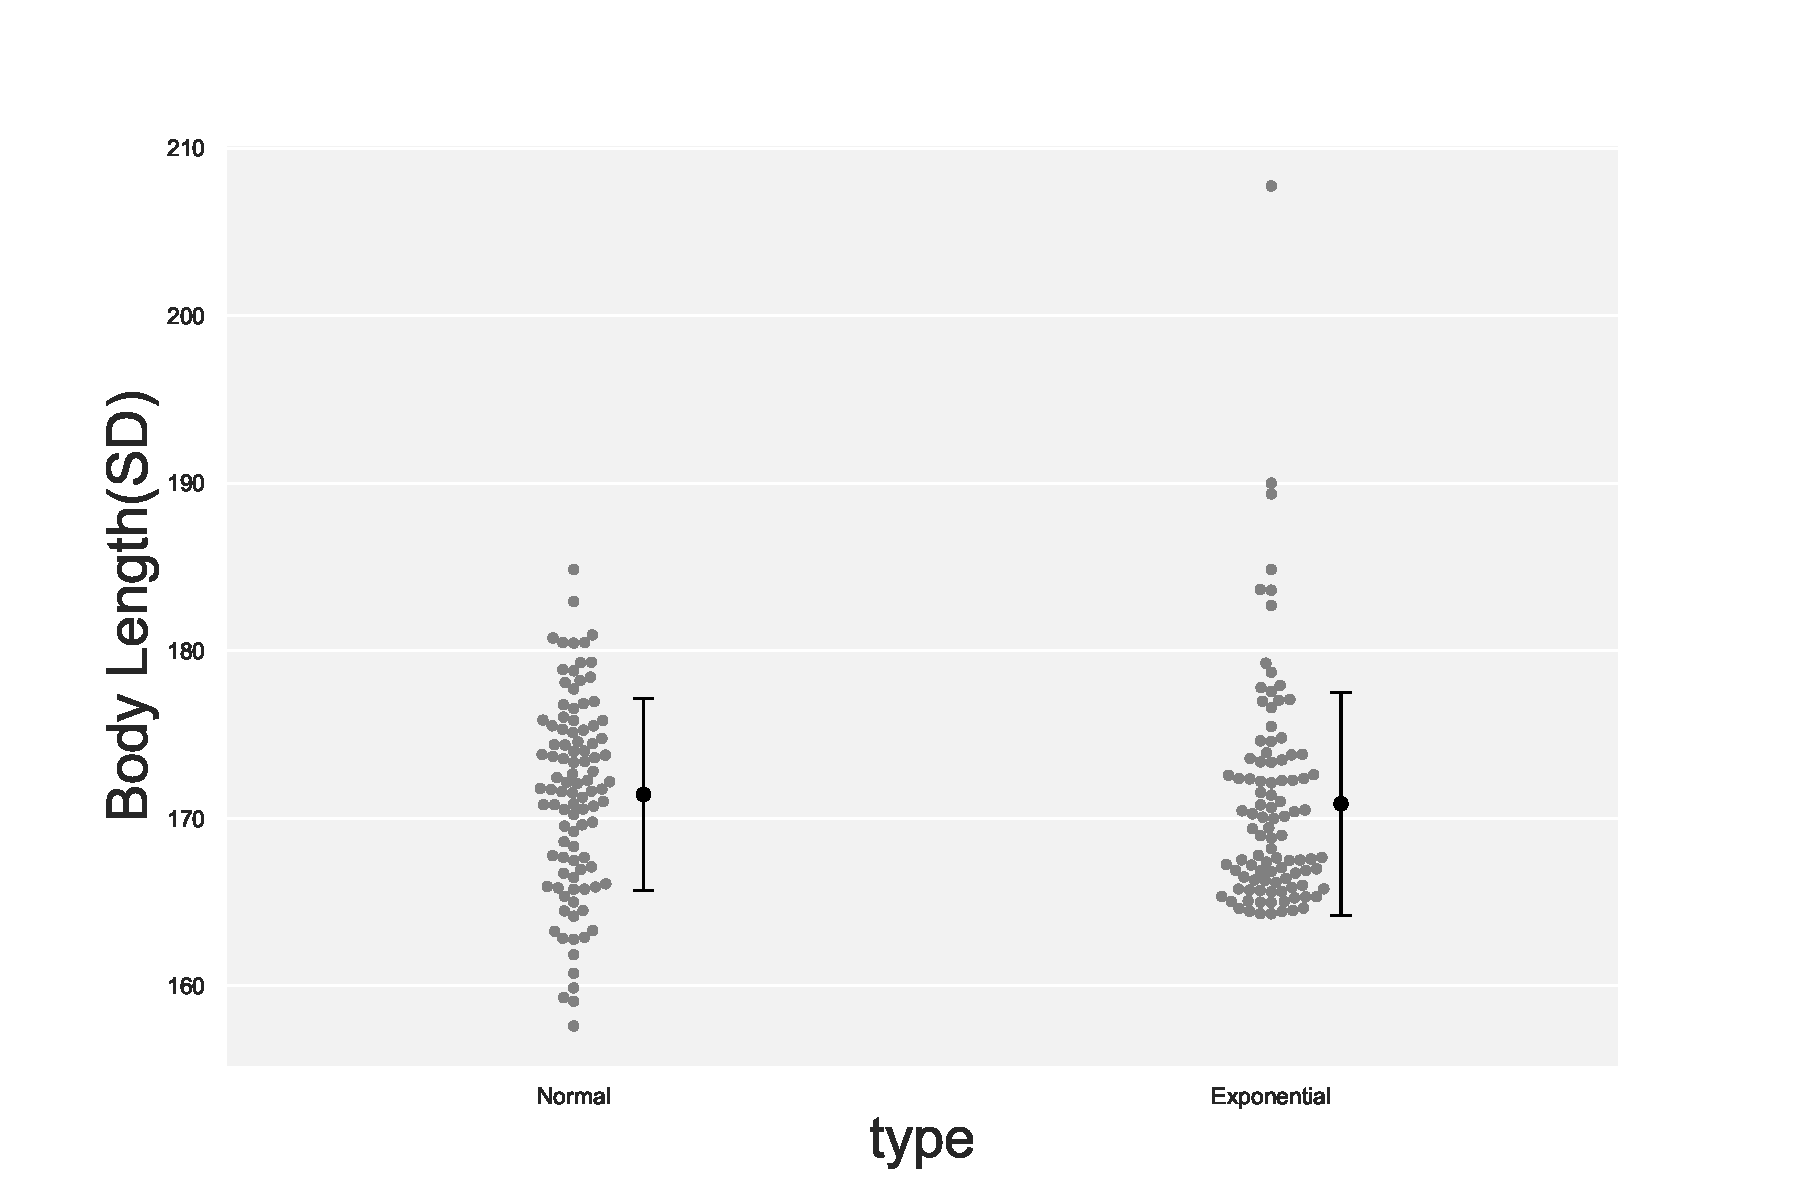
\includegraphics[width=15cm]{./image/12_/sample_norm_expon.pdf}
  \label{fig:sample_norm_expon_model}
  \caption{正規分布と指数分布それぞれからサンプルサイズ$N=100$の標本をプロットした。それぞれの右側にあるエラーバーは、正規分布モデルが予測した$68\%$予測区間。}
 \end{center}
\end{figure}


\begin{figure}
 \begin{center}
  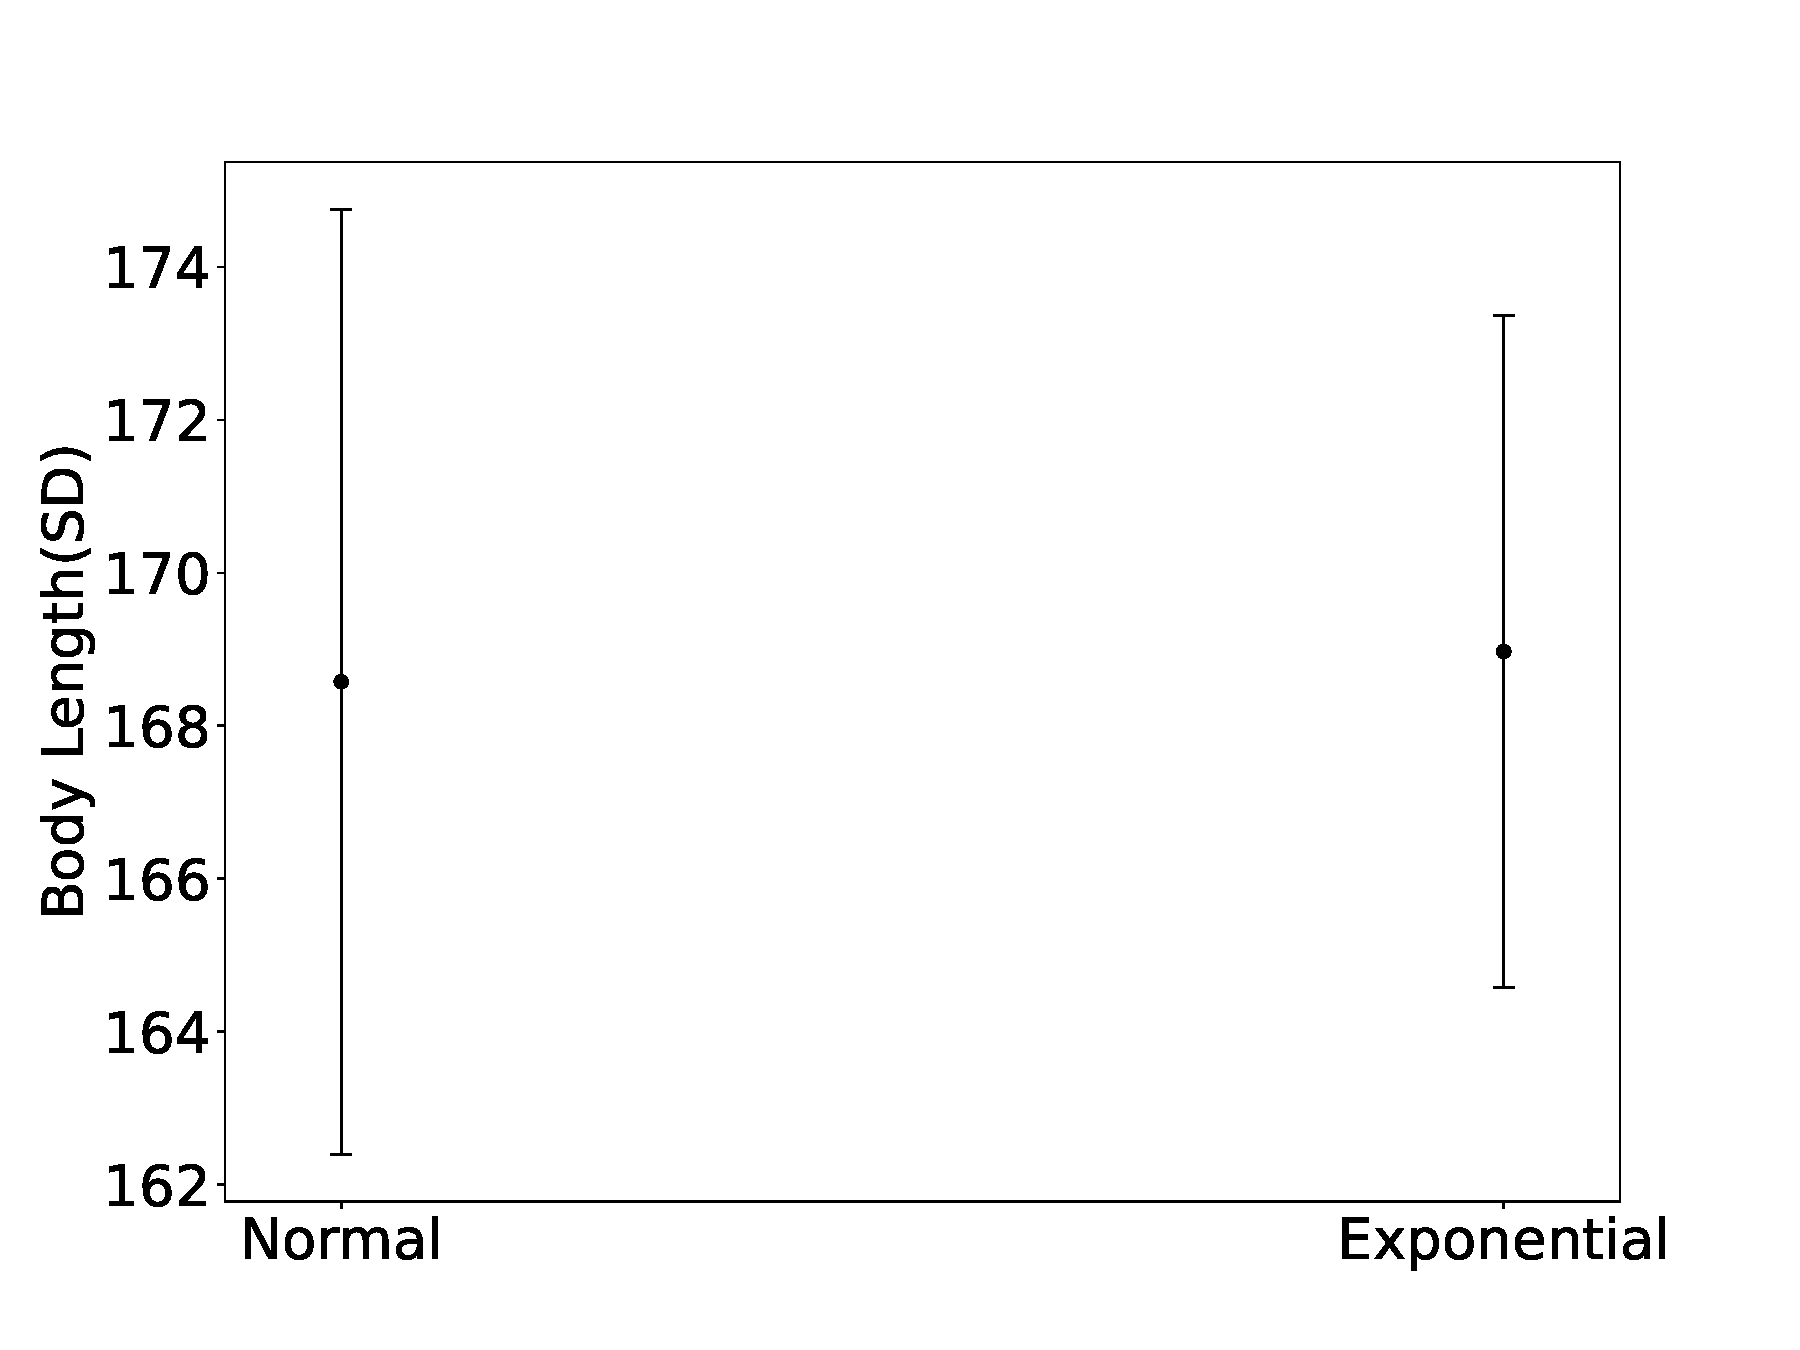
\includegraphics[width=15cm]{./image/12_/model_predict_SD.pdf}
  \label{fig:model_predict_SD}
  \caption{正規分布と指数分布それぞれからサンプルサイズ$N=100$の標本を得た。その標本から推測される$68\%$予測区間を描画した。}
 \end{center}
\end{figure}



\subsubsection{精度の良さを示すエラーバー}
測定精度の良さを示す指標としてSDを書くことがある。
この場合、ばらつき方は大抵正規分布的である。
また提案手法のSDがそれまでの計測方法よりも小さければ良い計測であるので、SDを表示している。


%\subsubsection{標本全体を使う方法}


%\section{良さそうなモデルをデータから選ぶ方法}



\section{累積分布によるデータとモデルの比較}

標本の累積分布のプロット方法について説明する。
標本$X_1,X_2,\cdots,X_n$を小さいものの順に並び替えたものを、$X_{r(1)},X_{r(2)},\cdots,X_{r(n)}$とする。ここで、$r(j)$は、$j$番目のデータのインデックスを返す関数である。
そして、
\begin{equation*}\label{commlative_rank_eq}
    (X_{r(j)},j/n) \ \ \ (j=1,2,\cdots,n)
\end{equation*}
をプロットする。
言い換えれば、累積分布は、標本を小さい順に並べたものと、順位をサンプルサイズで割ったもののペアをプロットしたものである。

具体的なコードは次のようになる
\begin{lstlisting}
def cummlative_norm(data):
    sorted_data = np.sort(data) # 順番の並び替え X_{r(j)}
    x = np.arange(len(data))/len(data) # データ数分のj/n 
    mu_ml,sigma_ml = np.mean(data),np.std(data)
    predict_cdf = norm(mu_ml,sigma_ml).cdf(sorted_data)
    return sorted_data,x,predict_cdf
\end{lstlisting}

\subsection{累積分布の傾き}
累積分布は、データの密集度が高い範囲において、傾きが大きくなり、密集度の小さい範囲では、傾きが小さくなる(図\ref{fig:qq_ccummlative_data_example_normummlative})。


\begin{figure}
 \begin{center}
  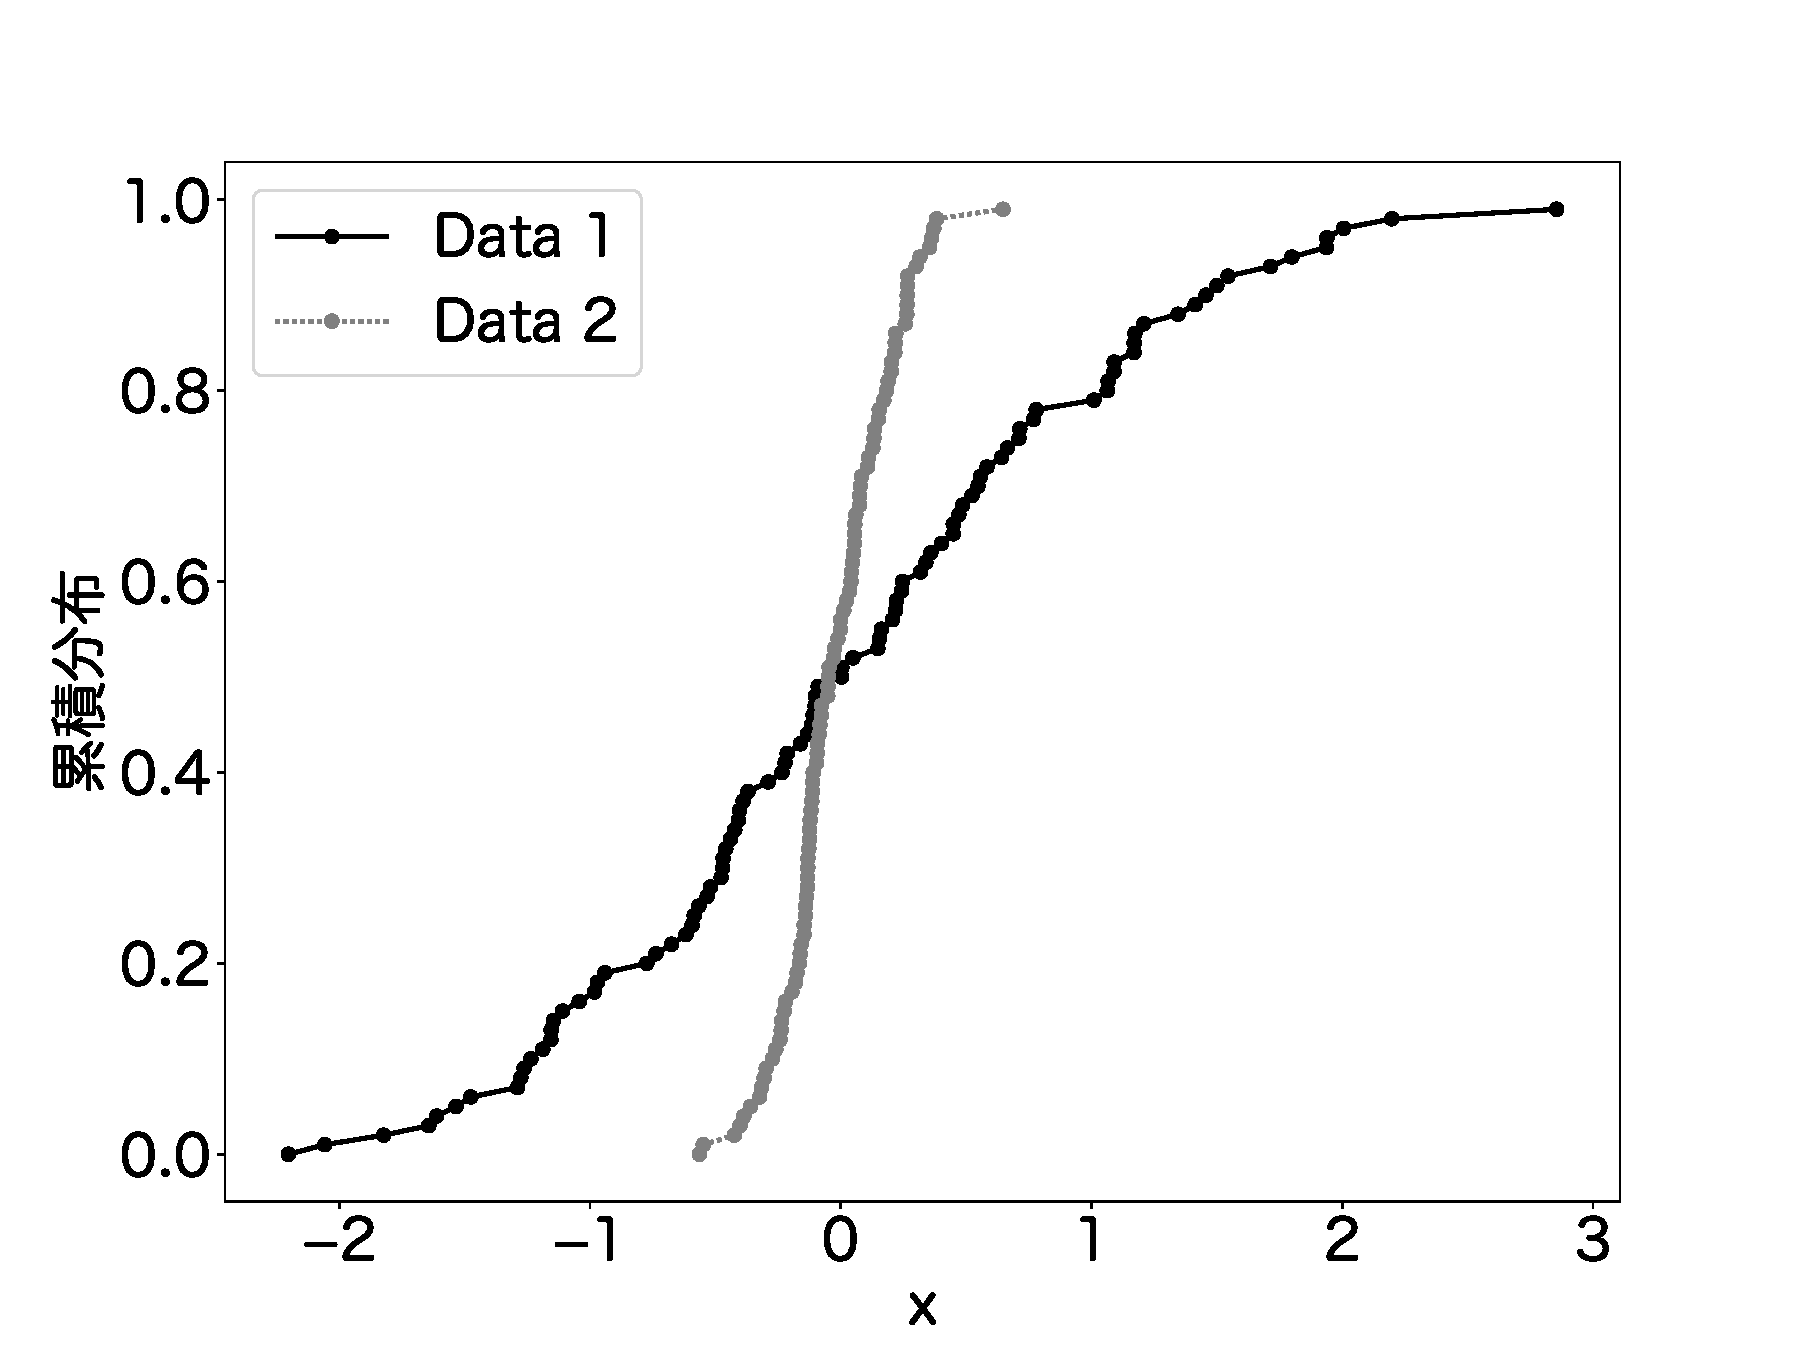
\includegraphics[width=15cm]{./image/12_/cummlative_data_example_norm.pdf}
  \label{fig:qq_ccummlative_data_example_normummlative}
  \caption{データの累積分布。Data 1は、正規分布$N(0,1)$、Data 2は正規分布$N(0,0.2)$からサンプリングした。サンプルサイズは$100$}
 \end{center}
\end{figure}


\subsection{データとモデルの比較}
図\ref{fig:qq_cummlative_30}図\ref{fig:qq_cummlative}右側に累積分布を描いておいた。
データは、(a)正規分布、(b)指数分布、(c)ガンマ分布からそれぞれサンプルサイズ$100$の標本である。
それぞれに、正規分布の最尤モデルを重ね書きしておいたので、最尤モデルとの乖離具合が把握できる。
(a)では、最尤正規モデルとデータが一致している。
(b,c)では、最尤正規モデルの曲線上に、データの累積分布の点が乗っていないので、モデルとデータが乖離していることが示唆される。
このことから、このようなデータが得られたなら、モデルを再構築したほうが良い。
また、サンプルサイズを30にした図\ref{fig:qq_cummlative_30}では、データが正規分布であっても、正規モデルによって推測することが良いのかはぱっと見では判断しにくく、正規モデルを確信を持って利用しにくくなる。

\section{qqプロットによるデータと正規分布の比較}
qqプロットについて説明する。
まず上記式\ref{commlative_rank_eq}について、$j/n$を、$F^{-1}(j/n)$によって逆変換する。ここで、累積標準正規分布の逆関数を$F^{-1}(p)$とする。
そして、$X_{r(j)}$と$F^{-1}(j/n)$の組
\begin{equation*}
(F^{-1}(j/n),X_{r(j)}) \ \ (j=0,1,\cdots,n)
\end{equation*}
をプロットする。これが$qq$プロットである。

\begin{lstlisting}
    def qq_plot(data,ax):
        sorted_data = np.array(sorted(data))
        p = np.arange(len(data))/len(data)
        x_ = norm(0,1).ppf(p)
        return np.c_[x_,sorted_data]
\end{lstlisting}


qqプロットを図\ref{fig:qq_cummlative_30}図\ref{fig:qq_cummlative}左側に描いた。直線に乗っているデータは、正規モデルの推測が当たりやすいと考えられる。

\begin{figure}
    \begin{center}
        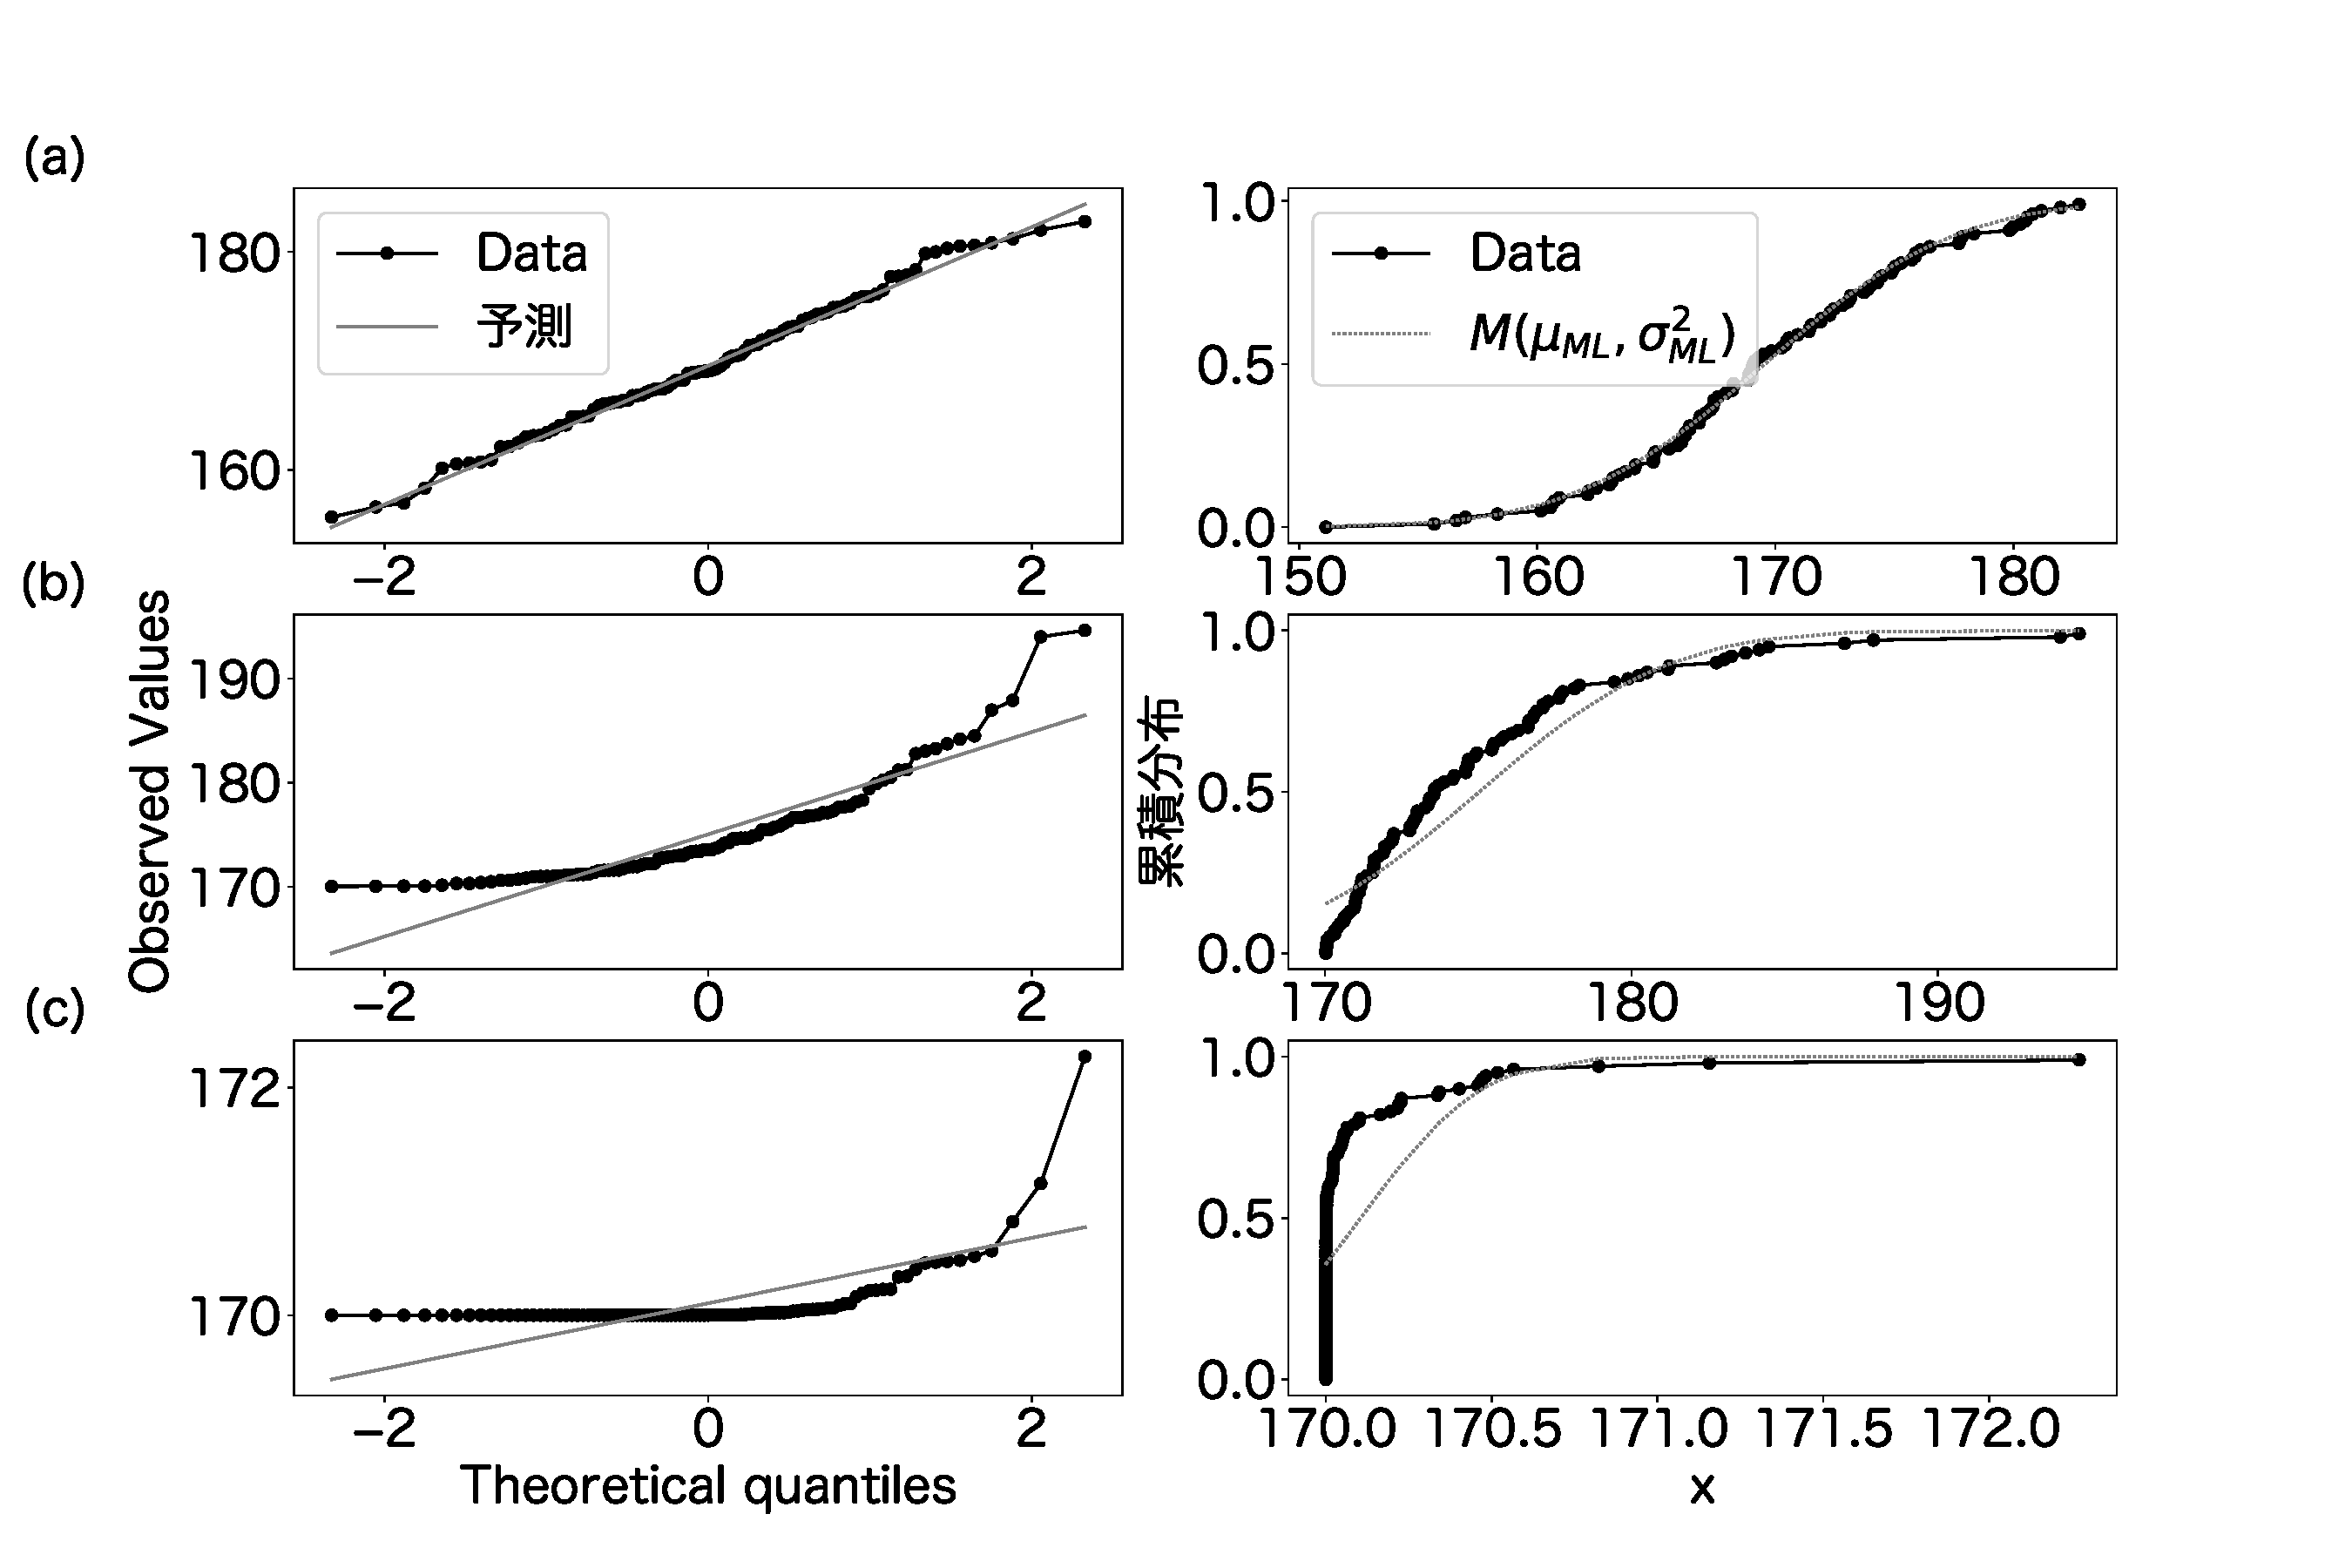
\includegraphics[width=15cm]{./image/12_/qq_cummlative_expon_norm_gamma.pdf}
        \label{fig:qq_cummlative}
        \caption{左にはqqプロット、右は累積分布と最尤モデルの累積分布。サンプルサイズは100(a)正規分布$N(170,5.8)$(b)指数分布$\lambda=5.8$(c)ガンマ分布$s=0.1$)}
    \end{center}
\end{figure}

\begin{figure}
 \begin{center}
  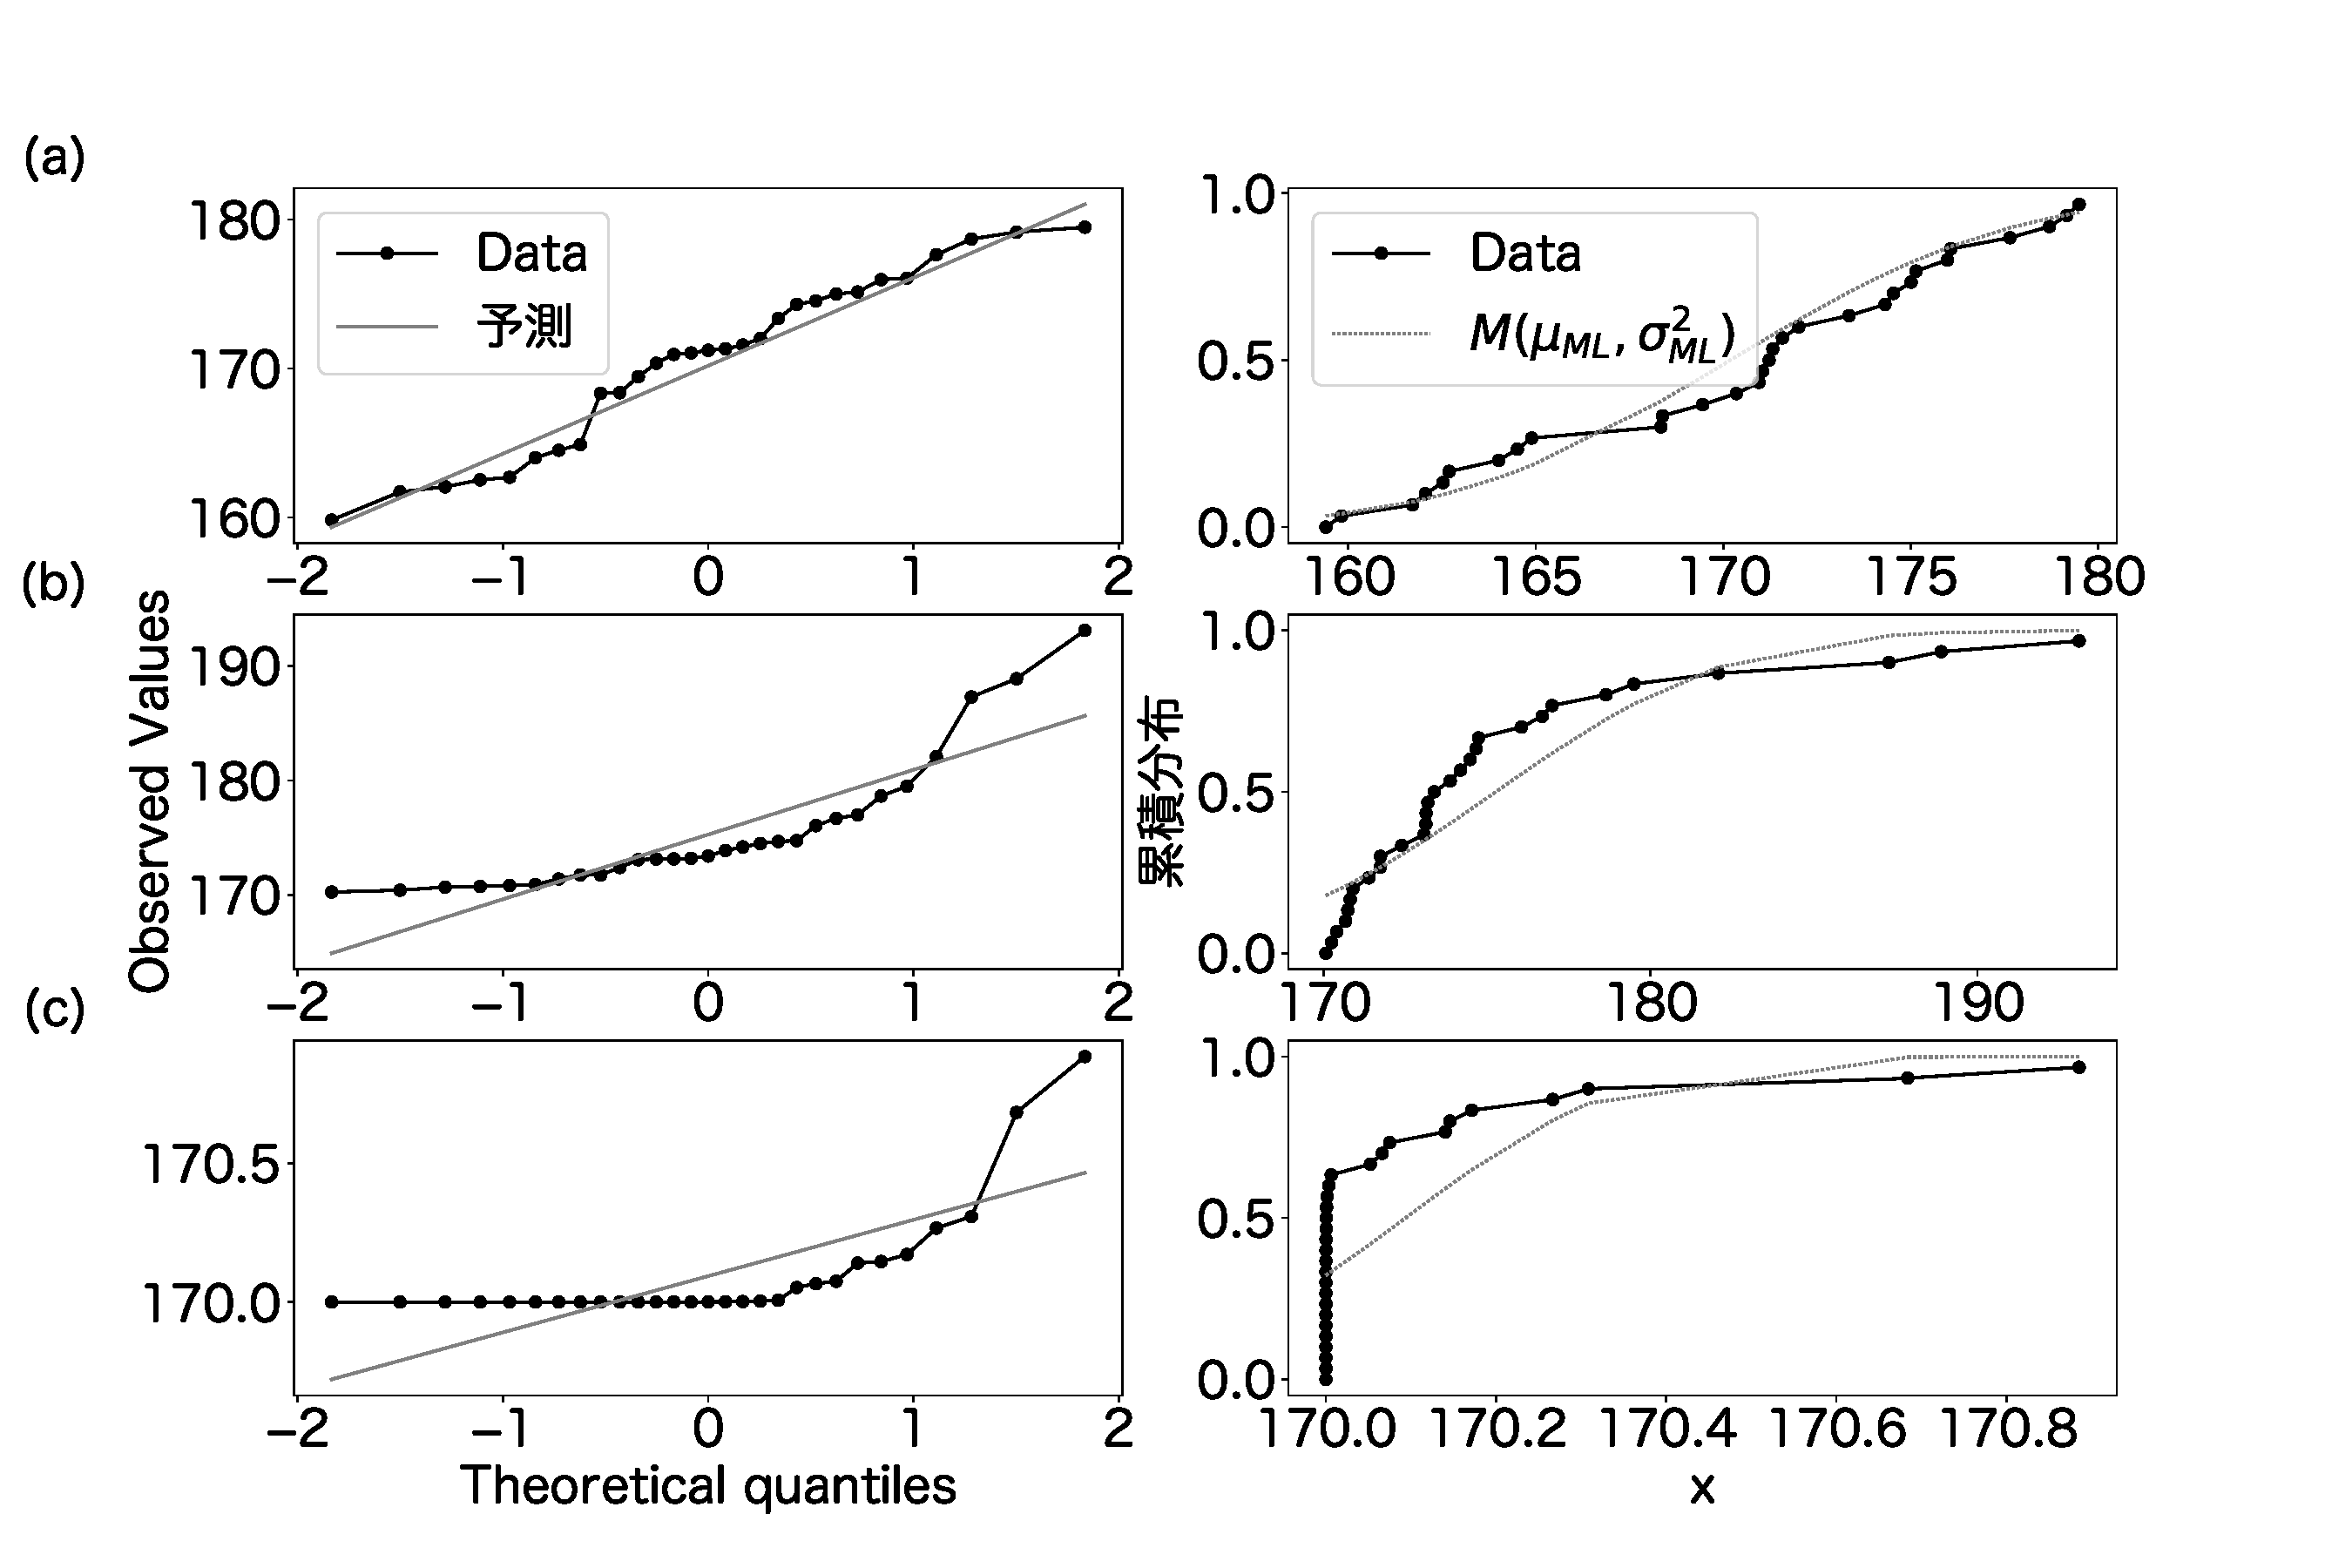
\includegraphics[width=15cm]{./image/12_/qq_cummlative_expon_norm_gammaN_30.pdf}
  \label{fig:qq_cummlative_30}
  \caption{左にはqqプロット、右は累積分布と最尤モデルの累積分布。サンプルサイズは30(a)正規分布$N(170,5.8)$(b)指数分布$\lambda=5.8$(c)ガンマ分布$s=0.1$)}
 \end{center}
\end{figure}

\section{AIC(相対的なモデルのデータへの適合具合)}
%\subsubsection{AICの比較}
AICは、対数尤度に対して、データ由来のパラメータ分、ペナルティを与えたものである。
AICが低いモデルは、相対的に良くデータに当てはまるモデルであり、そのモデルからデータが生成されたことを示唆するものではない。また、AICの差が$10$あったから良いとか悪いとかではなく、AICが低いものが相対的に良いモデルと判断されがちになるだけである。AICが小さいから、良い予測をすることが常にそうなるともかぎらない。

正規モデルのデータに対するAICを計算する。
母数を最尤推定により決定した最尤モデルのパラメータ数は2である\footnote{データ由来の母数2つあるので}。
例えば、過去の研究データから、平均$\mu$を決定し分散については最尤推定量により決定したモデル$M(\sigma^2_{ML})$のパラメータ数は$1$である。
% TODO: このパラメータ数は正しいのかがよくわからん。

%\subsubsection{AICが低いモデルは良い予測をするモデル?}
%AICが低いから、良い予測ができるかは不明である。
%一般に、比較対象のモデルの中で、データへの適合度が相対的に高いモデルである。
%まず、AICが低いモデルでも、データの出現を予測しにくい事例を紹介する。




